\pdfoutput=1
%% Author: PGL  Porta Mana, ALS Filipowicz
%% Created: 2018-04-08T16:54:19+0200
%% Last-Updated: 2018-07-05T20:01:50+0200
%%%%%%%%%%%%%%%%%%%%%%%%%%%%%%%%%%%%%%%%%%%%%%%%%%%%%%%%%%%%%%%%%%%%%%
% Report-no: ***
\newif\ifarxiv
\arxivfalse
\ifarxiv\pdfmapfile{+classico.map}\fi
\newif\ifafour
\afourfalse % true = A4, false = A5
\newif\iftypodisclaim % typographical disclaim on the side
\typodisclaimtrue
\newif\ifpublic
\publicfalse % true = for publication, false = personal notes
\newcommand*{\memfontfamily}{zplx}
\newcommand*{\memfontpack}{newpxtext}
\documentclass[\ifafour a4paper,12pt,\else a5paper,10pt,\fi%extrafontsizes,%
onecolumn,oneside,article,%french,italian,german,swedish,latin,
british%
]{memoir}
\newcommand*{\updated}{\today}
\newcommand*{\firstdraft}{14 April 2018}
\newcommand*{\firstpublished}{\today}
\newcommand*{\propertitle}{Bayesian Plinko\\{\large Study notes}}
\newcommand*{\pdftitle}{Bayesian Plinko}
\newcommand*{\headtitle}{Bayesian Plinko}
\newcommand*{\pdfauthor}{A. L. S. Filipowicz, P.G.L.  Porta Mana, Y. Roudi,
  Britt Anderson, James Danckert}
\newcommand*{\etal}{{et al.}}
\newcommand*{\headauthor}{\ifpublic Filipowicz \amp\ Porta Mana%
\else Alex \etal\fi}
\newcommand*{\reporthead}{}
%%%%%%%%%%%%%%%%%%%%%%%%%%%%%%%%%%%%%%%%%%%%%%%%%%%%%%%%%%%%%%%%%%%%%%%%%%%%
%%%%%%%%%%%%%%%%%%%%%%%%%%%%%%%%%%%%%%%%%%%%%%%%%%%%%%%%%%%%%%%%%%%%%%%%%%%%
%\usepackage{pifont}
%\usepackage{fontawesome}
\usepackage[T1]{fontenc} 
\input{glyphtounicode} \pdfgentounicode=1
\usepackage[utf8]{inputenx}
%\usepackage{newunicodechar}
% \newunicodechar{Ĕ}{\u{E}}
% \newunicodechar{ĕ}{\u{e}}
% \newunicodechar{Ĭ}{\u{I}}
% \newunicodechar{ĭ}{\u{\i}}
% \newunicodechar{Ŏ}{\u{O}}
% \newunicodechar{ŏ}{\u{o}}
% \newunicodechar{Ŭ}{\u{U}}
% \newunicodechar{ŭ}{\u{u}}
% \newunicodechar{Ā}{\=A}
% \newunicodechar{ā}{\=a}
% \newunicodechar{Ē}{\=E}
% \newunicodechar{ē}{\=e}
% \newunicodechar{Ī}{\=I}
% \newunicodechar{ī}{\={\i}}
% \newunicodechar{Ō}{\=O}
% \newunicodechar{ō}{\=o}
% \newunicodechar{Ū}{\=U}
% \newunicodechar{ū}{\=u}
% \newunicodechar{Ȳ}{\=Y}
% \newunicodechar{ȳ}{\=y}

\newcommand*{\bmmax}{0} % reduce number of bold fonts, before bm
\newcommand*{\hmmax}{0} % reduce number of heavy fonts, before bm
\usepackage{textcomp}
\usepackage[normalem]{ulem}
% \makeatletter
% \def\ssout{\bgroup \ULdepth=-.35ex%\UL@setULdepth
%  \markoverwith{\lower\ULdepth\hbox
%    {\kern-.03em\vbox{\hrule width.2em\kern1.2\p@\hrule}\kern-.03em}}%
%  \ULon}
% \makeatother
\usepackage{amsmath}
\usepackage{mathtools}
\addtolength{\jot}{\jot} % increase spacing in multiline formulae
\usepackage{empheq}% automatically calls amsmath and mathtools
\newcommand*{\widefbox}[1]{\fbox{\hspace{1em}#1\hspace{1em}}}
\setlength{\multlinegap}{0pt}
%\usepackage{fancybox}
%\usepackage{framed}
% \usepackage[misc]{ifsym} % for dice
% \newcommand*{\diceone}{{\scriptsize\Cube{1}}}
\usepackage{amssymb}
\usepackage{amsxtra}

\usepackage[main=british,french,italian,german,swedish,latin,esperanto]{babel}\selectlanguage{british}
\newcommand*{\langfrench}{\foreignlanguage{french}}
\newcommand*{\langgerman}{\foreignlanguage{german}}
\newcommand*{\langitalian}{\foreignlanguage{italian}}
\newcommand*{\langswedish}{\foreignlanguage{swedish}}
\newcommand*{\langlatin}{\foreignlanguage{latin}}
\newcommand*{\langnohyph}{\foreignlanguage{nohyphenation}}

\usepackage[autostyle=false,autopunct=false,english=british]{csquotes}
\setquotestyle{british}

\usepackage{amsthm}
\newcommand*{\QED}{\textsc{q.e.d.}}
\renewcommand*{\qedsymbol}{\QED}
\theoremstyle{remark}
\newtheorem{note}{Note}
\newtheorem*{remark}{Note}
\newtheoremstyle{innote}{\parsep}{\parsep}{\footnotesize}{}{}{}{0pt}{}
\theoremstyle{innote}
\newtheorem*{innote}{}


\usepackage[shortlabels,inline]{enumitem}
\SetEnumitemKey{para}{itemindent=\parindent,leftmargin=0pt,listparindent=\parindent,parsep=0pt,itemsep=\topsep}
% \begin{asparaenum} = \begin{enumerate}[para]
% \begin{inparaenum} = \begin{enumerate*}
\setlist[enumerate,2]{label=\alph*.}
\setlist[enumerate]{leftmargin=\parindent}
\setlist[itemize]{leftmargin=\parindent}
\setlist[description]{leftmargin=\parindent}

\usepackage[babel,theoremfont]{newpxtext}
\usepackage[bigdelims,nosymbolsc%,smallerops % probably arXiv doesn't have it
]{newpxmath}
\useosf\linespread{1.083}
%% smaller operators for old version of newpxmath
\makeatletter
\def\re@DeclareMathSymbol#1#2#3#4{%
    \let#1=\undefined
    \DeclareMathSymbol{#1}{#2}{#3}{#4}}
%\re@DeclareMathSymbol{\bigsqcupop}{\mathop}{largesymbols}{"46}
%\re@DeclareMathSymbol{\bigodotop}{\mathop}{largesymbols}{"4A}
\re@DeclareMathSymbol{\bigoplusop}{\mathop}{largesymbols}{"4C}
\re@DeclareMathSymbol{\bigotimesop}{\mathop}{largesymbols}{"4E}
\re@DeclareMathSymbol{\sumop}{\mathop}{largesymbols}{"50}
\re@DeclareMathSymbol{\prodop}{\mathop}{largesymbols}{"51}
\re@DeclareMathSymbol{\bigcupop}{\mathop}{largesymbols}{"53}
\re@DeclareMathSymbol{\bigcapop}{\mathop}{largesymbols}{"54}
%\re@DeclareMathSymbol{\biguplusop}{\mathop}{largesymbols}{"55}
\re@DeclareMathSymbol{\bigwedgeop}{\mathop}{largesymbols}{"56}
\re@DeclareMathSymbol{\bigveeop}{\mathop}{largesymbols}{"57}
%\re@DeclareMathSymbol{\bigcupdotop}{\mathop}{largesymbols}{"DF}
%\re@DeclareMathSymbol{\bigcapplusop}{\mathop}{largesymbolsPXA}{"00}
%\re@DeclareMathSymbol{\bigsqcupplusop}{\mathop}{largesymbolsPXA}{"02}
%\re@DeclareMathSymbol{\bigsqcapplusop}{\mathop}{largesymbolsPXA}{"04}
%\re@DeclareMathSymbol{\bigsqcapop}{\mathop}{largesymbolsPXA}{"06}
\re@DeclareMathSymbol{\bigtimesop}{\mathop}{largesymbolsPXA}{"10}
%\re@DeclareMathSymbol{\coprodop}{\mathop}{largesymbols}{"60}
%\re@DeclareMathSymbol{\varprod}{\mathop}{largesymbolsPXA}{16}
\makeatother


%% With euler font cursive for Greek letters - the [1] means 100% scaling
\DeclareFontFamily{U}{egreek}{\skewchar\font'177}%
\DeclareFontShape{U}{egreek}{m}{n}{<-6>s*[1]eurm5 <6-8>s*[1]eurm7 <8->s*[1]eurm10}{}%
\DeclareFontShape{U}{egreek}{m}{it}{<->s*[1]eurmo10}{}%
\DeclareFontShape{U}{egreek}{b}{n}{<-6>s*[1]eurb5 <6-8>s*[1]eurb7 <8->s*[1]eurb10}{}%
\DeclareFontShape{U}{egreek}{b}{it}{<->s*[1]eurbo10}{}%
\DeclareSymbolFont{egreeki}{U}{egreek}{m}{it}%
\SetSymbolFont{egreeki}{bold}{U}{egreek}{b}{it}% from the amsfonts package
\DeclareSymbolFont{egreekr}{U}{egreek}{m}{n}%
\SetSymbolFont{egreekr}{bold}{U}{egreek}{b}{n}% from the amsfonts package
% Take also \sum, \prod, \coprod symbols from Euler fonts
\DeclareFontFamily{U}{egreekx}{\skewchar\font'177}
\DeclareFontShape{U}{egreekx}{m}{n}{%
       <-7.5>s*[0.9]euex7%
    <7.5-8.5>s*[0.9]euex8%
    <8.5-9.5>s*[0.9]euex9%
    <9.5->s*[0.9]euex10%
}{}
\DeclareSymbolFont{egreekx}{U}{egreekx}{m}{n}
\DeclareMathSymbol{\sumop}{\mathop}{egreekx}{"50}
\DeclareMathSymbol{\prodop}{\mathop}{egreekx}{"51}
\DeclareMathSymbol{\coprodop}{\mathop}{egreekx}{"60}
\makeatletter
\def\sum{\DOTSI\sumop\slimits@}
\def\prod{\DOTSI\prodop\slimits@}
\def\coprod{\DOTSI\coprodop\slimits@}
\makeatother
\ifarxiv\else\let\varpartial\undefined
\let\partialup\undefined
\let\alpha\undefined
\let\beta\undefined
\let\gamma\undefined
\let\delta\undefined
\let\epsilon\undefined
\let\zeta\undefined
\let\eta\undefined
\let\theta\undefined
\let\iota\undefined
\let\kappa\undefined
\let\lambda\undefined
\let\mu\undefined
\let\nu\undefined
\let\xi\undefined
\let\omicron\undefined
\let\pi\undefined
\let\rho\undefined
\let\sigma\undefined
\let\tau\undefined
\let\upsilon\undefined
\let\phi\undefined
\let\chi\undefined
\let\psi\undefined
\let\omega\undefined
\let\varepsilon\undefined
\let\vartheta\undefined
\let\varpi\undefined
\let\varrho\undefined 
\let\varsigma\undefined
\let\varkappa\undefined
\let\varphi\undefined
%
\let\varAlpha\undefined
\let\varBeta\undefined
\let\varGamma\undefined
\let\varDelta\undefined
\let\varEpsilon\undefined
\let\varZeta\undefined
\let\varEta\undefined
\let\varTheta\undefined
\let\varIota\undefined
\let\varKappa\undefined
\let\varLambda\undefined
\let\varMu\undefined
\let\varNu\undefined
\let\varXi\undefined
\let\varOmicron\undefined
\let\varPi\undefined
\let\varRho\undefined
\let\varSigma\undefined
\let\varTau\undefined
\let\varUpsilon\undefined
\let\varPhi\undefined
\let\varChi\undefined
\let\varPsi\undefined
\let\varOmega\undefined
%
\let\Alpha\undefined
\let\Beta\undefined
\let\Gamma\undefined
\let\Delta\undefined
\let\Epsilon\undefined
\let\Zeta\undefined
\let\Eta\undefined
\let\Theta\undefined
\let\Iota\undefined
\let\Kappa\undefined
\let\Lambda\undefined
\let\Mu\undefined
\let\Nu\undefined
\let\Xi\undefined
\let\Omicron\undefined
\let\Pi\undefined
\let\Rho\undefined
\let\Sigma\undefined
\let\Tau\undefined
\let\Upsilon\undefined
\let\Phi\undefined
\let\Chi\undefined
\let\Psi\undefined
\let\Omega\undefined
%
\let\alphaup\undefined
\let\betaup\undefined
\let\gammaup\undefined
\let\deltaup\undefined
\let\epsilonup\undefined
\let\zetaup\undefined
\let\etaup\undefined
\let\thetaup\undefined
\let\iotaup\undefined
\let\kappaup\undefined
\let\lambdaup\undefined
\let\muup\undefined
\let\nuup\undefined
\let\xiup\undefined
\let\omicronup\undefined
\let\piup\undefined
\let\rhoup\undefined
\let\sigmaup\undefined
\let\tauup\undefined
\let\upsilonup\undefined
\let\phiup\undefined
\let\chiup\undefined
\let\psiup\undefined
\let\omegaup\undefined
\let\varepsilonup\undefined
\let\varthetaup\undefined
\let\varpiup\undefined
\let\varrhoup\undefined
\let\varsigmaup\undefined
\let\varkappaup\undefined
\let\varphiup\undefined
\fi% make sure no CMF greek letters sneak in
% Greek letters not usually given in LaTeX. Comment the unneeded ones
% \DeclareMathSymbol{\varpartial}{\mathalpha}{egreeki}{"40}
 \DeclareMathSymbol{\partialup}{\mathalpha}{egreekr}{"40}
% \DeclareMathSymbol{\alpha}{\mathalpha}{egreeki}{"0B}
% \DeclareMathSymbol{\beta}{\mathalpha}{egreeki}{"0C}
 \DeclareMathSymbol{\gamma}{\mathalpha}{egreeki}{"0D}
% \DeclareMathSymbol{\delta}{\mathalpha}{egreeki}{"0E}
 \DeclareMathSymbol{\epsilon}{\mathalpha}{egreeki}{"0F}
% \DeclareMathSymbol{\zeta}{\mathalpha}{egreeki}{"10}
% \DeclareMathSymbol{\eta}{\mathalpha}{egreeki}{"11}
 \DeclareMathSymbol{\theta}{\mathalpha}{egreeki}{"12}
% \DeclareMathSymbol{\iota}{\mathalpha}{egreeki}{"13}
 \DeclareMathSymbol{\kappa}{\mathalpha}{egreeki}{"14}
 \DeclareMathSymbol{\lambda}{\mathalpha}{egreeki}{"15}
 \DeclareMathSymbol{\mu}{\mathalpha}{egreeki}{"16}
 \DeclareMathSymbol{\nu}{\mathalpha}{egreeki}{"17}
% \DeclareMathSymbol{\xi}{\mathalpha}{egreeki}{"18}
% \DeclareMathSymbol{\omicron}{\mathalpha}{egreeki}{"6F}
% \DeclareMathSymbol{\pi}{\mathalpha}{egreeki}{"19}
% \DeclareMathSymbol{\rho}{\mathalpha}{egreeki}{"1A}
% \DeclareMathSymbol{\sigma}{\mathalpha}{egreeki}{"1B}
% \DeclareMathSymbol{\tau}{\mathalpha}{egreeki}{"1C}
% \DeclareMathSymbol{\upsilon}{\mathalpha}{egreeki}{"1D}
% \DeclareMathSymbol{\phi}{\mathalpha}{egreeki}{"1E}
 \DeclareMathSymbol{\chi}{\mathalpha}{egreeki}{"1F}
% \DeclareMathSymbol{\psi}{\mathalpha}{egreeki}{"20}
% \DeclareMathSymbol{\omega}{\mathalpha}{egreeki}{"21}
% \DeclareMathSymbol{\varepsilon}{\mathalpha}{egreeki}{"22}
% \DeclareMathSymbol{\vartheta}{\mathalpha}{egreeki}{"23}
% \DeclareMathSymbol{\varpi}{\mathalpha}{egreeki}{"24}
% \let\varrho\rho 
% \let\varsigma\sigma
 \let\varkappa\kappa
% \DeclareMathSymbol{\varphi}{\mathalpha}{egreeki}{"27}
% %
 \DeclareMathSymbol{\varAlpha}{\mathalpha}{egreeki}{"41}
 \DeclareMathSymbol{\varBeta}{\mathalpha}{egreeki}{"42}
% \DeclareMathSymbol{\varGamma}{\mathalpha}{egreeki}{"00}
 \DeclareMathSymbol{\varDelta}{\mathalpha}{egreeki}{"01}
 \DeclareMathSymbol{\varEpsilon}{\mathalpha}{egreeki}{"45}
% \DeclareMathSymbol{\varZeta}{\mathalpha}{egreeki}{"5A}
% \DeclareMathSymbol{\varEta}{\mathalpha}{egreeki}{"48}
 \DeclareMathSymbol{\varTheta}{\mathalpha}{egreeki}{"02}
 \DeclareMathSymbol{\varIota}{\mathalpha}{egreeki}{"49}
% \DeclareMathSymbol{\varKappa}{\mathalpha}{egreeki}{"4B}
 \DeclareMathSymbol{\varLambda}{\mathalpha}{egreeki}{"03}
% \DeclareMathSymbol{\varMu}{\mathalpha}{egreeki}{"4D}
% \DeclareMathSymbol{\varNu}{\mathalpha}{egreeki}{"4E}
% \DeclareMathSymbol{\varXi}{\mathalpha}{egreeki}{"04}
 \DeclareMathSymbol{\varOmicron}{\mathalpha}{egreeki}{"4F}
% \DeclareMathSymbol{\varPi}{\mathalpha}{egreeki}{"05}
% \DeclareMathSymbol{\varRho}{\mathalpha}{egreeki}{"50}
% \DeclareMathSymbol{\varSigma}{\mathalpha}{egreeki}{"06}
% \DeclareMathSymbol{\varTau}{\mathalpha}{egreeki}{"54}
% \DeclareMathSymbol{\varUpsilon}{\mathalpha}{egreeki}{"07}
% \DeclareMathSymbol{\varPhi}{\mathalpha}{egreeki}{"08}
% \DeclareMathSymbol{\varChi}{\mathalpha}{egreeki}{"58}
% \DeclareMathSymbol{\varPsi}{\mathalpha}{egreeki}{"09}
% \DeclareMathSymbol{\varOmega}{\mathalpha}{egreeki}{"0A} 
% %
% \DeclareMathSymbol{\Alpha}{\mathalpha}{egreekr}{"41}
% \DeclareMathSymbol{\Beta}{\mathalpha}{egreekr}{"42}
 \DeclareMathSymbol{\Gamma}{\mathalpha}{egreekr}{"00}
% \DeclareMathSymbol{\Delta}{\mathalpha}{egreekr}{"01}
% \DeclareMathSymbol{\Epsilon}{\mathalpha}{egreekr}{"45}
% \DeclareMathSymbol{\Zeta}{\mathalpha}{egreekr}{"5A}
% \DeclareMathSymbol{\Eta}{\mathalpha}{egreekr}{"48}
% \DeclareMathSymbol{\Theta}{\mathalpha}{egreekr}{"02}
% \DeclareMathSymbol{\Iota}{\mathalpha}{egreekr}{"49}
% \DeclareMathSymbol{\Kappa}{\mathalpha}{egreekr}{"4B}
% \DeclareMathSymbol{\Lambda}{\mathalpha}{egreekr}{"03}
% \DeclareMathSymbol{\Mu}{\mathalpha}{egreekr}{"4D}
% \DeclareMathSymbol{\Nu}{\mathalpha}{egreekr}{"4E}
% \DeclareMathSymbol{\Xi}{\mathalpha}{egreekr}{"04}
% \DeclareMathSymbol{\Omicron}{\mathalpha}{egreekr}{"4F}
% \DeclareMathSymbol{\Pi}{\mathalpha}{egreekr}{"05}
% \DeclareMathSymbol{\Rho}{\mathalpha}{egreekr}{"50}
% \DeclareMathSymbol{\Sigma}{\mathalpha}{egreekr}{"06}
% \DeclareMathSymbol{\Tau}{\mathalpha}{egreekr}{"54}
% \DeclareMathSymbol{\Upsilon}{\mathalpha}{egreekr}{"07}
% \DeclareMathSymbol{\Phi}{\mathalpha}{egreekr}{"08}
% \DeclareMathSymbol{\Chi}{\mathalpha}{egreekr}{"58}
% \DeclareMathSymbol{\Psi}{\mathalpha}{egreekr}{"09}
% \DeclareMathSymbol{\Omega}{\mathalpha}{egreekr}{"0A}
% %
% \DeclareMathSymbol{\alphaup}{\mathalpha}{egreekr}{"0B}
% \DeclareMathSymbol{\betaup}{\mathalpha}{egreekr}{"0C}
% \DeclareMathSymbol{\gammaup}{\mathalpha}{egreekr}{"0D}
 \DeclareMathSymbol{\deltaup}{\mathalpha}{egreekr}{"0E}
% \DeclareMathSymbol{\epsilonup}{\mathalpha}{egreekr}{"0F}
% \DeclareMathSymbol{\zetaup}{\mathalpha}{egreekr}{"10}
% \DeclareMathSymbol{\etaup}{\mathalpha}{egreekr}{"11}
% \DeclareMathSymbol{\thetaup}{\mathalpha}{egreekr}{"12}
% \DeclareMathSymbol{\iotaup}{\mathalpha}{egreekr}{"13}
% \DeclareMathSymbol{\kappaup}{\mathalpha}{egreekr}{"14}
% \DeclareMathSymbol{\lambdaup}{\mathalpha}{egreekr}{"15}
% \DeclareMathSymbol{\muup}{\mathalpha}{egreekr}{"16}
% \DeclareMathSymbol{\nuup}{\mathalpha}{egreekr}{"17}
% \DeclareMathSymbol{\xiup}{\mathalpha}{egreekr}{"18}
% \DeclareMathSymbol{\omicronup}{\mathalpha}{egreekr}{"6F}
  \DeclareMathSymbol{\piup}{\mathalpha}{egreekr}{"19}
% \DeclareMathSymbol{\rhoup}{\mathalpha}{egreekr}{"1A}
 \DeclareMathSymbol{\sigmaup}{\mathalpha}{egreekr}{"1B}
% \DeclareMathSymbol{\tauup}{\mathalpha}{egreekr}{"1C}
% \DeclareMathSymbol{\upsilonup}{\mathalpha}{egreekr}{"1D}
% \DeclareMathSymbol{\phiup}{\mathalpha}{egreekr}{"1E}
% \DeclareMathSymbol{\chiup}{\mathalpha}{egreekr}{"1F}
% \DeclareMathSymbol{\psiup}{\mathalpha}{egreekr}{"20}
% \DeclareMathSymbol{\omegaup}{\mathalpha}{egreekr}{"21}
% \DeclareMathSymbol{\varepsilonup}{\mathalpha}{egreekr}{"22}
% \DeclareMathSymbol{\varthetaup}{\mathalpha}{egreekr}{"23}
% \DeclareMathSymbol{\varpiup}{\mathalpha}{egreekr}{"24}
% \let\varrhoup\rhoup 
% \let\varsigmaup\sigmaup
% \let\varkappaup\kappaup
% \DeclareMathSymbol{\varphiup}{\mathalpha}{egreekr}{"27}

% Optima as sans-serif font
%\usepackage%[scaled=0.9]%
%{classico}
\renewcommand\sfdefault{uop}
\DeclareMathAlphabet{\mathsf}  {T1}{\sfdefault}{m}{sl}
\SetMathAlphabet{\mathsf}{bold}{T1}{\sfdefault}{b}{sl}
\newcommand*{\mathte}[1]{\textbf{\textit{\textsf{#1}}}}
% Upright sans-serif math alphabet
% \DeclareMathAlphabet{\mathsu}  {T1}{\sfdefault}{m}{n}
% \SetMathAlphabet{\mathsu}{bold}{T1}{\sfdefault}{b}{n}

% DejaVu Mono as typewriter text
\usepackage[scaled=0.84]{DejaVuSansMono}


\usepackage{mathdots}

\usepackage[usenames]{xcolor}
% Tol (2012) colour-blind-, print-, screen-friendly colours; Munsell terminology
\definecolor{mybluishpurple}{RGB}{51,34,136}
\definecolor{myblue}{RGB}{136,204,238}
\definecolor{mybluishgreen}{RGB}{68,170,153}
\definecolor{mygreen}{RGB}{17,119,51}
\definecolor{mygreenishyellow}{RGB}{153,153,51}
\definecolor{myyellow}{RGB}{221,204,119}
\definecolor{myred}{RGB}{204,102,119}
\definecolor{mypurplishred}{RGB}{136,34,85}
\definecolor{myreddishpurple}{RGB}{170,68,153}
\definecolor{mygrey}{RGB}{221,221,221}
%\newcommand*\mycolourbox[1]{%
%\colorbox{mygrey}{\hspace{1em}#1\hspace{1em}}}
\colorlet{shadecolor}{mygrey}

\usepackage{bm}
\usepackage{microtype}

\usepackage[backend=biber,mcite,%subentry,
citestyle=authoryear-comp,bibstyle=pglpm-authoryear,autopunct=false,sorting=ny,sortcites=false,natbib=false,maxcitenames=1,maxbibnames=8,minbibnames=8,giveninits=true,uniquename=false,uniquelist=false,maxalphanames=1,block=space,hyperref=true,defernumbers=false,useprefix=true,sortupper=false,language=british,parentracker=false]{biblatex}
\DeclareSortingScheme{ny}{\sort{\field{sortname}\field{author}\field{editor}}\sort{\field{year}}}
\iffalse\makeatletter%%% replace parenthesis with brackets
\newrobustcmd*{\parentexttrack}[1]{%
  \begingroup
  \blx@blxinit
  \blx@setsfcodes
  \blx@bibopenparen#1\blx@bibcloseparen
  \endgroup}
\AtEveryCite{%
  \let\parentext=\parentexttrack%
  \let\bibopenparen=\bibopenbracket%
  \let\bibcloseparen=\bibclosebracket}
\makeatother\fi
\DefineBibliographyExtras{british}{\def\finalandcomma{\addcomma}}
\renewcommand*{\finalnamedelim}{\addcomma\space}
\setcounter{biburlnumpenalty}{1}
\setcounter{biburlucpenalty}{0}
\setcounter{biburllcpenalty}{1}
\DeclareDelimFormat{multicitedelim}{\addsemicolon\space}
\DeclareDelimFormat{compcitedelim}{\addsemicolon\space}
\DeclareDelimFormat{postnotedelim}{\space}
\ifarxiv\else\addbibresource{portamanabib.bib}\fi
\renewcommand{\bibfont}{\footnotesize}
%\appto{\citesetup}{\footnotesize}% smaller font for citations
\defbibheading{bibliography}[\bibname]{\section*{#1}\addcontentsline{toc}{section}{#1}%\markboth{#1}{#1}
}
\newcommand*{\citep}{\parencites}
\newcommand*{\citey}{\parencites*}
%\renewcommand*{\cite}{\parencite}
\renewcommand*{\cites}{\parencites}
\providecommand{\href}[2]{#2}
\providecommand{\eprint}[2]{\texttt{\href{#1}{#2}}}
\newcommand*{\amp}{\&}
% \newcommand*{\citein}[2][]{\textnormal{\textcite[#1]{#2}}%\addtocategory{extras}{#2}
% }
\newcommand*{\citein}[2][]{\textnormal{\textcite[#1]{#2}}%\addtocategory{extras}{#2}
}
\newcommand*{\citebi}[2][]{\textcite[#1]{#2}%\addtocategory{extras}{#2}
}
\newcommand*{\subtitleproc}[1]{}
\newcommand*{\chapb}{ch.}

% \def\arxivp{}
% \def\mparcp{}
% \def\philscip{}
% \def\biorxivp{}
% \newcommand*{\arxivsi}{\texttt{arXiv} eprints available at \url{http://arxiv.org/}.\\}
% \newcommand*{\mparcsi}{\texttt{mp\_arc} eprints available at \url{http://www.ma.utexas.edu/mp_arc/}.\\}
% \newcommand*{\philscisi}{\texttt{philsci} eprints available at \url{http://philsci-archive.pitt.edu/}.\\}
% \newcommand*{\biorxivsi}{\texttt{bioRxiv} eprints available at \url{http://biorxiv.org/}.\\}
\newcommand*{\arxiveprint}[1]{%\global\def\arxivp{\arxivsi}%\citeauthor{0arxivcite}\addtocategory{ifarchcit}{0arxivcite}%eprint
\texttt{\urlalt{https://arxiv.org/abs/#1}{arXiv:\hspace{0pt}#1}}%
%\texttt{\href{http://arxiv.org/abs/#1}{\protect\url{arXiv:#1}}}%
%\renewcommand{\arxivnote}{\texttt{arXiv} eprints available at \url{http://arxiv.org/}.}
}
\newcommand*{\mparceprint}[1]{%\global\def\mparcp{\mparcsi}%\citeauthor{0mparccite}\addtocategory{ifarchcit}{0mparccite}%eprint
\texttt{\urlalt{http://www.ma.utexas.edu/mp_arc-bin/mpa?yn=#1}{mp\_arc:\hspace{0pt}#1}}%
%\texttt{\href{http://www.ma.utexas.edu/mp_arc-bin/mpa?yn=#1}{\protect\url{mp_arc:#1}}}%
%\providecommand{\mparcnote}{\texttt{mp_arc} eprints available at \url{http://www.ma.utexas.edu/mp_arc/}.}
}
\newcommand*{\philscieprint}[1]{%\global\def\philscip{\philscisi}%\citeauthor{0philscicite}\addtocategory{ifarchcit}{0philscicite}%eprint
\texttt{\urlalt{http://philsci-archive.pitt.edu/archive/#1}{PhilSci:\hspace{0pt}#1}}%
%\texttt{\href{http://philsci-archive.pitt.edu/archive/#1}{\protect\url{PhilSci:#1}}}%
%\providecommand{\mparcnote}{\texttt{philsci} eprints available at \url{http://philsci-archive.pitt.edu/}.}
}
\newcommand*{\biorxiveprint}[1]{%\global\def\biorxivp{\biorxivsi}%\citeauthor{0arxivcite}\addtocategory{ifarchcit}{0arxivcite}%eprint
\texttt{\urlalt{http://biorxiv.org/content/early/#1}{bioRxiv:\hspace{0pt}#1}}%
%\texttt{\href{http://arxiv.org/abs/#1}{\protect\url{arXiv:#1}}}%
%\renewcommand{\arxivnote}{\texttt{arXiv} eprints available at \url{http://arxiv.org/}.}
}
\newcommand*{\osfeprint}[1]{%
\texttt{\urlalt{https://doi.org/10.17605/osf.io/#1}{doi:10.17605/osf.io/#1}}%
}

\usepackage{graphicx}
\usepackage{wrapfig}

\PassOptionsToPackage{hyphens}{url}\usepackage[hypertexnames=false]{hyperref}
\usepackage[depth=4]{bookmark}
\hypersetup{colorlinks=true,bookmarksnumbered,pdfborder={0 0 0.25},citebordercolor={0.2 0.1333 0.5333},%bluish
citecolor=mybluishpurple,linkbordercolor={0.0667 0.4667 0.2},%greenish
linkcolor=mypurplishred,urlbordercolor={0.5333 0.1333 0.3333},%reddish
urlcolor=mygreen,breaklinks=true,pdftitle={\pdftitle},pdfauthor={\pdfauthor}}
% \usepackage[vertfit=local]{breakurl}% only for arXiv
\providecommand*{\urlalt}{\href}

%%% Layout. I do not know on which kind of paper the reader will print the
%%% paper on (A4? letter? one-sided? double-sided?). So I choose A5, which
%%% provides a good layout for reading on screen and save paper if printed
%%% two pages per sheet. Average length line is 66 characters and page
%%% numbers are centred.
\ifafour\setstocksize{297mm}{210mm}%{*}% A4
\else\setstocksize{210mm}{5.5in}%{*}% 210x139.7
\fi
\settrimmedsize{\stockheight}{\stockwidth}{*}
\setlxvchars[\normalfont] %313.3632pt for a 66-characters line
\setxlvchars[\normalfont]
\setlength{\trimtop}{0pt}
\setlength{\trimedge}{\stockwidth}
\addtolength{\trimedge}{-\paperwidth}
% The length of the normalsize alphabet is 133.05988pt - 10 pt = 26.1408pc
% The length of the normalsize alphabet is 159.6719pt - 12pt = 30.3586pc
% Bringhurst gives 32pc as boundary optimal with 69 ch per line
% The length of the normalsize alphabet is 191.60612pt - 14pt = 35.8634pc
\ifafour\settypeblocksize{*}{32pc}{1.618} % A4
%\setulmargins{*}{*}{1.667}%gives 5/3 margins % 2 or 1.667
\else\settypeblocksize{*}{26pc}{1.618}% nearer to a 66-line newpx and preserves GR
\fi
\setulmargins{*}{*}{1}%gives equal margins
\setlrmargins{*}{*}{*}
\setheadfoot{\onelineskip}{2.5\onelineskip}
\setheaderspaces{*}{2\onelineskip}{*}
\setmarginnotes{2ex}{10mm}{0pt}
\checkandfixthelayout[nearest]
\fixpdflayout
%%% End layout
%% this fixes missing white spaces
\pdfmapline{+dummy-space <dummy-space.pfb}\pdfinterwordspaceon%

%%% Sectioning
\newcommand*{\asudedication}[1]{%
{\par\centering\textit{#1}\par}}
\newenvironment{acknowledgements}{\section*{Thanks}\addcontentsline{toc}{section}{Thanks}}{\par}
\makeatletter\renewcommand{\appendix}{\par
  \bigskip{\centering
   \interlinepenalty \@M
   \normalfont
   \printchaptertitle{\sffamily\appendixpagename}\par}
  \setcounter{section}{0}%
  \gdef\@chapapp{\appendixname}%
  \gdef\thesection{\@Alph\c@section}%
  \anappendixtrue}\makeatother
\counterwithout{section}{chapter}
\setsecnumformat{\upshape\csname the#1\endcsname\quad}
\setsecheadstyle{\large\bfseries\sffamily%
\raggedright}
\setsubsecheadstyle{\bfseries\sffamily%
\raggedright}
%\setbeforesecskip{-1.5ex plus 1ex minus .2ex}% plus 1ex minus .2ex}
%\setaftersecskip{1.3ex plus .2ex }% plus 1ex minus .2ex}
%\setsubsubsecheadstyle{\bfseries\sffamily\slshape\raggedright}
%\setbeforesubsecskip{1.25ex plus 1ex minus .2ex }% plus 1ex minus .2ex}
%\setaftersubsecskip{-1em}%{-0.5ex plus .2ex}% plus 1ex minus .2ex}
\setsubsecindent{0pt}%0ex plus 1ex minus .2ex}
\setparaheadstyle{\bfseries\sffamily%
\raggedright}
\setcounter{secnumdepth}{2}
\setlength{\headwidth}{\textwidth}
\newcommand{\addchap}[1]{\chapter*[#1]{#1}\addcontentsline{toc}{chapter}{#1}}
\newcommand{\addsec}[1]{\section*{#1}\addcontentsline{toc}{section}{#1}}
\newcommand{\addsubsec}[1]{\subsection*{#1}\addcontentsline{toc}{subsection}{#1}}
\newcommand{\addpara}[1]{\paragraph*{#1.}\addcontentsline{toc}{subsubsection}{#1}}
\newcommand{\addparap}[1]{\paragraph*{#1}\addcontentsline{toc}{subsubsection}{#1}}

% Headers and footers
\copypagestyle{manaart}{plain}
\makeheadrule{manaart}{\headwidth}{0.5\normalrulethickness}
\makeoddhead{manaart}{%
{\footnotesize%\sffamily%
\scshape\headauthor}}{}{{\footnotesize\sffamily%
\headtitle}}
\makeoddfoot{manaart}{}{\thepage}{}
\newcommand*\autanet{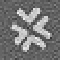
\includegraphics[height=\heightof{M}]{autanet.pdf}}
\definecolor{mygray}{gray}{0.333}
\iftypodisclaim%
\ifafour\newcommand\addprintnote{\begin{picture}(0,0)%
\put(245,149){\makebox(0,0){\rotatebox{90}{\tiny\color{mygray}\textsf{This
            document is designed for screen reading and
            two-up printing on A4 or Letter paper}}}}%
\end{picture}}% A4
\else\newcommand\addprintnote{\begin{picture}(0,0)%
\put(176,112){\makebox(0,0){\rotatebox{90}{\tiny\color{mygray}\textsf{This
            document is designed for screen reading and
            two-up printing on A4 or Letter paper}}}}%
\end{picture}}\fi%afourtrue
\makeoddfoot{plain}{}{\makebox[0pt]{\thepage}\addprintnote}{}
\else
\makeoddfoot{plain}{}{\makebox[0pt]{\thepage}}{}
\fi%typodisclaimtrue
\makeoddhead{plain}{}{}{\footnotesize\reporthead}

% \copypagestyle{manainitial}{plain}
% \makeheadrule{manainitial}{\headwidth}{0.5\normalrulethickness}
% \makeoddhead{manainitial}{%
% \footnotesize\sffamily%
% \scshape\headauthor}{}{\footnotesize\sffamily%
% \headtitle}
% \makeoddfoot{manaart}{}{\thepage}{}

\pagestyle{manaart}

\setlength{\droptitle}{-3.9\onelineskip}
\pretitle{\begin{center}\LARGE\sffamily%
\bfseries}
\posttitle{\bigskip\end{center}}

\makeatletter\newcommand*{\atf}{
\includegraphics[%trim=1pt 1pt 0pt 0pt,
totalheight=\heightof{@}]{atblack.png}}\makeatother
\providecommand{\affiliation}[1]{\textsl{\textsf{\footnotesize #1}}}
\providecommand{\epost}[1]{\texttt{\footnotesize\textless#1\textgreater}}
\providecommand{\email}[2]{\href{mailto:#1ZZ@#2 ((remove ZZ))}{#1\protect\atf#2}}

\preauthor{\vspace{-0.5\baselineskip}\begin{center}
\normalsize\sffamily%
\lineskip  0.5em}
\postauthor{\par\end{center}}
\predate{\DTMsetdatestyle{mydate}\begin{center}\footnotesize}
\postdate{\end{center}\vspace{-\medskipamount}}
\usepackage[british]{datetime2}
\DTMnewdatestyle{mydate}%
{% definitions
\renewcommand*{\DTMdisplaydate}[4]{%
\number##3\ \DTMenglishmonthname{##2} ##1}%
\renewcommand*{\DTMDisplaydate}{\DTMdisplaydate}%
}
\DTMsetdatestyle{mydate}


\setfloatadjustment{figure}{\footnotesize}
\captiondelim{\quad}
\captionnamefont{\footnotesize\sffamily%
}
\captiontitlefont{\footnotesize}
\firmlists*
\midsloppy

% handling orphan/widow lines, memman.pdf
% \clubpenalty=10000
% \widowpenalty=10000
% \raggedbottom
% Downes, memman.pdf
\clubpenalty=9996
\widowpenalty=9999
\brokenpenalty=4991
\predisplaypenalty=10000
\postdisplaypenalty=1549
\displaywidowpenalty=1602

\selectlanguage{british}\frenchspacing
%%%%%%%%%%%%%%%%%%%%%%%%%%%%%%%%%%%%%%%%%%%%%%%%%%%%%%%%%%%%%%%%%%%%%%%%%%%%
%%%%%%%%%%%%%%%%%%%%%%%%%%%%%%%%%%%%%%%%%%%%%%%%%%%%%%%%%%%%%%%%%%%%%%%%%%%%
%%%% Paper's details %%%%
\title{\propertitle%\\
%  {\large A geometric commentary on maximum-entropy proofs}% ***
}
\author{\ifpublic\hspace*{\stretch{1}}%
%\begin{tabular}[t]{c}
\parbox[t]{0.3\linewidth}{\protect\centering%
Alex\\%
{\footnotesize\epost{\email{alsfilip}{mail.med.penn.edu}}}}%
%\end{tabular}&%
\hspace*{\stretch{1}}%
%\begin{tabular}[t]{c}
\parbox[t]{0.3\linewidth}{\protect\centering%
P.G.L. Porta\,Mana\\%
{\footnotesize%\ \href{https://orcid.org/0000-0002-6070-0784}{\protect\includegraphics[scale=0.16]{orcid_32x32.png}}}\\{\footnotesize
\epost{\email{pgl}{portamana.org}}}%
}% \\%
% {\footnotesize\href{https://orcid.org/0000-0002-6070-0784}{\protect\includegraphics[scale=0.16]{orcid_32x32.png}\textsc{orcid}:0000-0002-6070-0784}}%
%\end{tabular}%
\hspace*{\stretch{1}}%
\else Alex, Luca, Yasser, Britt, James%
\fi}

%\date{\firstpublished; updated \updated}
\date{\firstdraft; updated \updated}

%\date{\firstpublished; updated \oggi}

%@@@@@@@@@@ new macros @@@@@@@@@@
% Common ones - uncomment as needed
%\providecommand{\nequiv}{\not\equiv}
%\providecommand{\coloneqq}{\mathrel{\mathop:}=}
%\providecommand{\eqqcolon}{=\mathrel{\mathop:}}
%\providecommand{\varprod}{\prod}
\newcommand*{\de}{\partialup}%partial diff
\newcommand*{\pu}{\piup}%constant pi
\newcommand*{\delt}{\deltaup}%Kronecker, Dirac
%\newcommand*{\eps}{\varepsilonup}%Levi-Civita, Heaviside
%\newcommand*{\riem}{\zetaup}%Riemann zeta
%\providecommand{\degree}{\textdegree}% degree
%\newcommand*{\celsius}{\textcelsius}% degree Celsius
%\newcommand*{\micro}{\textmu}% degree Celsius
%\newcommand*{\I}{\mathrm{i}}%imaginary unit
\newcommand*{\e}{\mathrm{e}}%Neper
\newcommand*{\di}{\mathrm{d}}%differential
%\newcommand*{\Di}{\mathrm{D}}%capital differential
%\newcommand*{\planckc}{\hslash}
%\newcommand*{\avogn}{N_{\textrm{A}}}
%\newcommand*{\NN}{\bm{\mathrm{N}}}
%\newcommand*{\ZZ}{\bm{\mathrm{Z}}}
%\newcommand*{\QQ}{\bm{\mathrm{Q}}}
\newcommand*{\RR}{\bm{\mathrm{R}}}
%\newcommand*{\CC}{\bm{\mathrm{C}}}
%\newcommand*{\nabl}{\bm{\nabla}}%nabla
%\DeclareMathOperator{\lb}{lb}%base 2 log
%\DeclareMathOperator{\tr}{tr}%trace
%\DeclareMathOperator{\card}{card}%cardinality
%\DeclareMathOperator{\im}{Im}%im part
%\DeclareMathOperator{\re}{Re}%re part
%\DeclareMathOperator{\sgn}{sgn}%signum
%\DeclareMathOperator{\ent}{ent}%integer less or equal to
%\DeclareMathOperator{\Ord}{O}%same order as
%\DeclareMathOperator{\ord}{o}%lower order than
%\newcommand*{\incr}{\triangle}%finite increment
\newcommand*{\defd}{\coloneqq}
\newcommand*{\defs}{\eqqcolon}
%\newcommand*{\Land}{\bigwedge}
%\newcommand*{\Lor}{\bigvee}
%\newcommand*{\lland}{\mathbin{\ \land\ }}
%\newcommand*{\llor}{\mathbin{\ \lor\ }}
%\newcommand*{\lonlyif}{\mathbin{\Rightarrow}}%implies
\newcommand*{\limplies}{\mathbin{\Rightarrow}}%implies
\newcommand*{\mimplies}{\Rightarrow}%implies
%\newcommand*{\liff}{\mathbin{\Leftrightarrow}}%if and only if
%\newcommand*{\cond}{\mathpunct{|}}%conditional sign (in probabilities)
%\newcommand*{\lcond}{\mathpunct{|\ }}%conditional sign (in probabilities)
%\newcommand*{\bigcond}{\mathpunct{\big|}}%conditional sign (in probabilities)
%\newcommand*{\lbigcond}{\mathpunct{\big|\ }}%conditional sign (in probabilities)
\newcommand*{\suchthat}{\mid}%{\mathpunct{|}}%such that (eg in sets)
%\newcommand*{\bigst}{\mathpunct{\big|}}%such that (eg in sets)
%\newcommand*{\with}{\colon}%with (list of indices)
%\newcommand*{\mul}{\times}%multiplication
%\newcommand*{\inn}{\cdot}%inner product
%\newcommand*{\dotv}{\mathord{\,\cdot\,}}%variable place
%\newcommand*{\comp}{\circ}%composition of functions
%\newcommand*{\con}{\mathbin{:}}%scal prod of tensors
%\newcommand*{\equi}{\sim}%equivalent to 
\renewcommand*{\asymp}{\simeq}%equivalent to 
%\newcommand*{\corr}{\mathrel{\hat{=}}}%corresponds to
%\providecommand{\varparallel}{\ensuremath{\mathbin{/\mkern-7mu/}}}%parallel (tentative symbol)
\renewcommand{\le}{\leqslant}%less or equal
\renewcommand{\ge}{\geqslant}%greater or equal
\DeclarePairedDelimiter\clcl{[}{]}
\DeclarePairedDelimiter\clop{[}{[}
%\DeclarePairedDelimiter\opcl{]}{]}
%\DeclarePairedDelimiter\opop{]}{[}
%\DeclarePairedDelimiter\abs{\lvert}{\rvert}
%\DeclarePairedDelimiter\norm{\lVert}{\rVert}
\DeclarePairedDelimiter\set{\{}{\}}
%\DeclareMathOperator{\pr}{P}%probability
\newcommand*{\pf}{\mathrm{p}}%probability
\newcommand*{\p}{\mathrm{P}}%probability
%\newcommand*{\tf}{\mathrm{T}}%probability
\renewcommand*{\|}{\mathpunct{|}}
%\newcommand*{\lcond}{\mathpunct{|\ }}%conditional sign (in probabilities)
\newcommand*{\bigcond}{\mathpunct{\big|\ }}%conditional sign (in probabilities)
%\newcommand*{\lbigcond}{\mathpunct{\big|\ }}%conditional sign (in probabilities)
%\newcommand*{\+}{\lor}
%\renewcommand{\*}{\land}
\newcommand*{\sect}{\S}% Sect.~
\newcommand*{\sects}{\S\S}% Sect.~
\newcommand*{\chap}{ch.}%
\newcommand*{\chaps}{chs}%
\newcommand*{\bref}{ref.}%
\newcommand*{\brefs}{refs}%
%\newcommand*{\fn}{fn}%
\newcommand*{\eqn}{eq.}%
\newcommand*{\eqns}{eqs}%
\newcommand*{\fig}{fig.}%
\newcommand*{\figs}{figs}%
\newcommand*{\vs}{{vs.}}
\newcommand*{\etc}{{etc.}}
\newcommand*{\ie}{{i.e.}}
%\newcommand*{\ca}{{c.}}
\newcommand*{\eg}{{e.g.}}
\newcommand*{\foll}{{ff.}}
%\newcommand*{\viz}{{viz}}
\newcommand*{\cf}{{cf.}}
%\newcommand*{\Cf}{{Cf.}}
%\newcommand*{\vd}{{v.}}
%\newcommand*{\etsim}{{et sim.}}
%\newcommand*{\ibid}{{ibid.}}
%\newcommand*{\sic}{{sic}}
%\newcommand*{\id}{\mathte{I}}%id matrix
%\newcommand*{\nbd}{\nobreakdash}%
%\newcommand*{\bd}{\hspace{0pt}}%
%\def\hy{-\penalty0\hskip0pt\relax}
\newcommand*{\labelbis}[1]{\tag*{(\ref{#1})$_\text{r}$}}
%\newcommand*{\mathbox}[2][.8]{\parbox[t]{#1\columnwidth}{#2}}
%\newcommand*{\zerob}[1]{\makebox[0pt][l]{#1}}
\newcommand*{\tprod}{\mathop{\textstyle\prod}\nolimits}
\newcommand*{\tsum}{\mathop{\textstyle\sum}\nolimits}
%\newcommand*{\tint}{\begingroup\textstyle\int\endgroup\nolimits}
%\newcommand*{\tland}{\mathop{\textstyle\bigwedge}\nolimits}
%\newcommand*{\tlor}{\mathop{\textstyle\bigvee}\nolimits}
%\newcommand*{\sprod}{\mathop{\textstyle\prod}}
%\newcommand*{\ssum}{\mathop{\textstyle\sum}}
%\newcommand*{\sint}{\begingroup\textstyle\int\endgroup}
%\newcommand*{\sland}{\mathop{\textstyle\bigwedge}}
%\newcommand*{\slor}{\mathop{\textstyle\bigvee}}
%\newcommand*{\T}{^\intercal}%transpose
%\newcommand*{\E}{\mathrm{E}}
%\DeclarePairedDelimiter\expp{(}{)}
%\newcommand*{\expe}{\E\expp}%round
%\newcommand*{\expeb}{\E\clcl}%square
%%\newcommand*{\QEM}%{\textnormal{$\Box$}}%{\ding{167}}
%\newcommand*{\qem}{\leavevmode\unskip\penalty9999 \hbox{}\nobreak\hfill
%\quad\hbox{\QEM}}

\definecolor{notecolour}{RGB}{68,170,153}
%\newcommand*{\puzzle}{{\fontencoding{U}\fontfamily{fontawesometwo}\selectfont\symbol{225}}}
\newcommand*{\puzzle}{\maltese}
\newcommand{\mynote}[1]{ {\color{notecolour}\puzzle\ #1\ }}
%\newcommand*{\widebar}[1]{{\mkern1.5mu\skew{2}\overline{\mkern-1.5mu#1\mkern-1.5mu}\mkern 1.5mu}}

%\DeclareMathOperator*{\argsup}{arg\,sup}
\newcommand*{\ptext}[1]{\text{\small #1}}
\newcommand*{\simpl}{\varDelta}
\newcommand*{\yqq}{q}
\newcommand*{\yq}{\bm{\yqq}}
\newcommand*{\yff}{f}
\newcommand*{\yf}{\bm{\yff}}
\newcommand*{\yI}{\varIota}
\newcommand*{\yO}{\varOmicron}
\newcommand*{\yIp}{\yI_{\textrm{p}}}
\newcommand*{\yMJ}{\yI_1}
\newcommand*{\yMc}{\yI_2}
\newcommand*{\yN}{\varLambda}
\newcommand*{\yNo}[1]{\yN^{(#1)}}
\newcommand*{\ynn}{\nu}
\newcommand*{\yn}{\bm{\nu}}
\newcommand*{\yno}[1]{\yn^{(#1)}}
\newcommand*{\ynno}[1]{\ynn^{(#1)}}
\newcommand*{\yth}{\theta}
\newcommand*{\yTh}{\varTheta}
\newcommand*{\ymu}{\mu}
\newcommand*{\yh}{\chi}
\newcommand*{\yrs}{h}
\newcommand*{\yc}{\gamma}
\newcommand*{\ycs}{\gamma_{\textrm{v}}}
\newcommand*{\ycm}{\gamma_{\textrm{m}}}
%\DeclareMathOperator{\logistic}{logistic}
\newcommand*{\logistic}{\sigmaup}
\AtBeginEnvironment{tabularx}{\setlist[enumerate]{wide, leftmargin=*,
    itemsep=0pt%, before=\vspace{-\dimexpr\baselineskip +2 \partopsep},
    % after=\vspace{-\baselineskip}
  }}
%@@@@@@@@@@ new macros end @@@@@@@@@@

\firmlists
\begin{document}
\captiondelim{\quad}\captionnamefont{\footnotesize}\captiontitlefont{\footnotesize}
\selectlanguage{british}\frenchspacing

%%% Title and abstract %%%
\maketitle
\ifpublic
\abstractrunin
\abslabeldelim{}
\renewcommand*{\abstractname}{}
\setlength{\absleftindent}{0pt}
\setlength{\absrightindent}{0pt}
\setlength{\abstitleskip}{-\absparindent}
\begin{abstract}\labelsep 0pt%
  \noindent How does a Bayesian robot do at Plinko, using an infinitely
  exchangeable model and borrowing a human participant's prior?
% \par%\\[\jot]
% \noindent
% {\footnotesize PACS: ***}\qquad%
% {\footnotesize MSC: ***}%
%\qquad{\footnotesize Keywords: ***}
\end{abstract}\fi

\selectlanguage{british}\frenchspacing
% \asudedication{\small ***}
% \vspace{\bigskipamount}

% \setlength{\epigraphwidth}{.7\columnwidth}
% \setlength{\epigraphrule}{0pt}
% \epigraphfontsize{\footnotesize}%
\setlength{\epigraphwidth}{.6\columnwidth}
%\epigraphposition{flushright}
\epigraphtextposition{flushright}
%\epigraphsourceposition{flushright}
\epigraphfontsize{\footnotesize}
\setlength{\epigraphrule}{0pt}
\setlength{\beforeepigraphskip}{0pt}
\setlength{\afterepigraphskip}{0pt}
\epigraph{We are human, after all\\
  Much in common, after all}{\citep{daftpunk2005b}}
%\vspace{-1em}
% \epigraph{If people always felt obliged to back their opinions when
%   challenged, we would be spared a few of the ``certain'' predictions that
%   are so freely made.}{\citep{good1950}}


% \noindent\emph{\footnotesize Note: Dear Peer, this manuscript is
%   peer-reviewed by \emph{you}. I'm grateful if you let me know of any
%   faults in its premisses, logic, evidence, and of any other criticisms you
%   may have.}


\section{Remarks, comments, thoughts on the project}
\label{sec:method_remarks}

\subsection{[Luca] What goes on in a participant's head? Possible models}

The experimental setup is open to a huge number of analyses and
interpretations on the participants' part, inspired by past experience. As
participants we can surmise that there's a connection between different
trials, some sort of \enquote{constant mechanism} at some level. Or we can
surmise that there's no such connection, hence observation of past trials
doesn't say anything about the next one. Or we can surmise that the next
trial is influenced by our own past probability assignments, recorded in
previous observations. And many other hypotheses. We can also entertain all
these hypotheses at the same time, and shift from one to another during the
experiment. For example, if we suddenly wondered whether the computer
program is actually using our past distributions, we could suddenly move
all probability to a slot at the edge and check if this seems to influence
the next outcome (\cf\ participant~31).

The same goes for the choice of initial distribution. As participants we
can say \enquote{alright, there are 40 slots}, and just give a uniform
distributions to the 40 possibilities. Or we can consider the pyramidal
mechanism of the game, which leads to a binomial distribution. Or we can
consider that this is a computerized version of the game. The computer
could simulate the physics of the actual game; but the image of the
mechanism could also be deceptive, the computer being programmed to
distribute the outcomes according to a predetermined, completely arbitrary
distribution. From this point of view we could again decide to assign a
uniform distribution.

\subsection{[Luca] Paradigms for judgement and assessment}

The literature I've seen so far explains at length how the data presented
to participants are generated, and is very succinct in explaining what was
said to the participants before the experiment. The participant's
inferences are then compared against models based on the pseudo-random
algorithm that generated the data. Nassar \etal's \citey{nassaretal2010}
work is an example.

I think that we should use a different paradigm to describe the experiment
and assess the participants' behaviours.

As I see it, the participants' inferential behaviours should be compared
with that of a \enquote{robot} that uses exact or approximate Bayesian or
decision-theoretic rules, and that \emph{starts from the same information
  that was given to the participants}. So it's really important that this
information be explained at length, and whatever the participants were told
should be reported verbatim.

I don't see the rationale of comparing a participant who doesn't know the
data-generating algorithm, with a robot that does. Such a robot is
modelling a different initial state of knowledge. What's important here,
instead, is to model the inference, given the same initial knowledge.

A consequence of this point of view is that there isn't just one robot that
can model the inferences. The information given to the participants is
never enough to make numeric inferences and apply the probability calculus:
it must always be augmented with additional assumptions, determined by each
participant's previous life experiences. Different robots can thus be
constructed: they use the same initial information as the participants, but
each is augmented with different auxiliary assumptions. \emph{The} ideal
observer doesn't exist. There are several ideal observers.

Another consequence of this point of view is that the data-generating
algorithm becomes slightly less important. The robot is constructed based
on the exact information given the participants, and uses the same data
given to the participants. The data-generating algorithm nowhere enters in
the construction of the robot.

\iffalse
De~Finetti introduced the notion of exchangeability in order to avoid
thinking in terms of \enquote{mechanisms} or of \enquote{true unknown
  distributions} \citep[\cf][\chap~3]{good1965}. He characterized a
statistical model in terms of \emph{features of the predictive
  distribution} -- for example, that it be invariant under exchanges of the
outcomes. This point of view was taken up by many other statisticians and
has been used to characterize many other statistical models, like Markov
ones for example
\citep{freedman1962,diaconisetal1980c,zaman1984,fortinietal2002,fortinietal2014}.
\fi


\section{The Bayesian robot}
\label{sec:bayesian_robot}

\subsection{A prosopopoeia of statistical models}
\label{sec:prosopopoeia}

A \emph{statistical model} can be defined as a set of assumptions that
allow us to make all possible numeric probabilistic inferences in the
context of an experiment or of a sequence of observations. These
assumptions correspond to -- indeed they're the exact generalization of --
axioms in propositional logic
\citep{hailperin1996,hailperin2011,jaynes1994_r2003}. Without axioms we
can't derive theorems with the logical calculus; without initial
probabilistic assumptions we can't derive or update probabilities with the
probability calculus.

Consider this context: a set of $M$ observations $1,2,\dotsc,M$, each of
which can have $N$ possible slot outcomes $\set{1,\dotsc,N}$. Denote
\enquote{The outcome of the $i$th \textbf{o}bservation is slot $s$} by
$\yO^i_s$, and logical conjunction (\enquote{$\land$}) by a comma.
In this context, choosing a statistical model $\yI$ is equivalent to
choosing the numerical values of the joint distribution
\begin{multline}
  \label{eq:distr_statmodel}
  \p( \yO^M_{s_M}, \yO^{M-1}_{s_{M-1}}, \dotsc,
  \yO^2_{s_2}, \yO^1_{s_1} \|  \yI)
  \quad\text{for all $s_1,\dotsc,s_M$}\\\text{(\ie, $N^M-1$ values)}
\end{multline}
for all combinations of $s_1,\dotsc,s_M \in \set{1,\dotsc,N}$; or to
choosing any other probabilistic assignments equivalent to this
distribution. An equivalent alternative, for example, is to assign the
distribution for the first observation:
\begin{subequations}
  \begin{align}
    &\p(\yO^1_{s_1} \|\yI)
    \quad\text{all $s_1$} &&\text{($N-1$ values)},
\\\intertext{the $N$ distributions for the second
  observation conditional on all possible first outcomes:}
    &\p(\yO^2_{s_2} \|\yO^1_{s_1}, \yI)
    \quad\text{all $s_1,s_2$} &&\text{($(N-1)\times N$ values)},
    \\
    \intertext{and so on up to the
  $N^{M-1}$ distributions for the $M$th observation conditional on all
  possible previous outcomes:}
&\p(\yO^M_{s_M} \|
\yO^{M-1}_{s_{M-1}},\dotsc,\yO^1_{s_1},\yI)
\quad\text{all $s_1,\dotsc,s_M$} &&\text{($(N-1)\times N^{M-1}$ values)}
  \end{align}
\end{subequations}
The product of these distributions is the joint
distribution~\eqref{eq:distr_statmodel}, and conversely each of these
distributions can be obtained from the joint one above by marginalization
and condizionalization.

Our assumptions can have different natures and motivations, for example
from symmetry, mechanics, biology. As long as they lead to definite
numerical values for the distribution above, they constitute a statistical
model.

The term \enquote{statistical model} is not universally used this way,
though.\footnote{\enquote{The conflict regarding the existence of a or the
    true model, model uncertainty, identification, selection,
    misspecification, etc.\ can be resolved if a clear definition of a
    model is stated. Models have different meanings in different fields.
    Once a young woman was interviewed for a data handling job in Unilever.
    She was puzzled by one of the interviewers who asked her whether she
    had done any modelling. It was found later that to her the question
    meant whether she had posed for photographs!} J. R. M. Ameen
  \citep[p.~453]{copasetal1995}.} It often has a more general meaning --
what we'd call \enquote{classes of statistical models} in our terminology.

To avoid using this ambiguous term, we'll figuratively speak of a
\emph{Bayesian robot} instead of a model. Such a robot uses the three,
five, or six laws of probability for negation, disjunction, conjunction,
implication:
\begin{subequations}
    \label{eq:laws_prob}
  \begin{gather}
\p(\neg \varAlpha \| \yI) = 1-\p(\varAlpha \| \yI)\\    
\p(\varAlpha, \varBeta \| \yI) =\p(\varBeta, \varAlpha \| \yI) = \p(\varAlpha \| \varBeta,\yI)\;\p(\varBeta \| \yI)\\
\p(\varAlpha \lor \varBeta \| \yI) =\p(\varBeta \lor \varAlpha \| \yI) = \p(\varAlpha \| \yI)+\p(\varBeta \| \yI)-\p(\varAlpha \| \varBeta,\yI)\;\p(\varBeta \| \yI)\\    
\p(\varAlpha\limplies \varBeta\|I) = \p(\neg \varAlpha \| \yI) +\p(\varAlpha \| \varBeta,\yI)\;\p(\varBeta \| \yI)
  \end{gather}
\end{subequations}
(the last three equalities are unnecessary if we define
$\varAlpha\lor \varBeta \defd \neg(\neg \varAlpha, \neg \varBeta)$ and
$\varAlpha \limplies \varBeta \defd \neg(\varAlpha, \neg \varBeta)$) to make numeric probabilistic
inferences and update them in view of new observations. But to do so it
first needs to be fully programmed with a complete set of probabilistic
assumptions, in the form of the joint
distribution~\eqref{eq:distr_statmodel} or in another equivalent way.
\emph{A \enquote{Bayesian robot} is thus equivalent to a statistical
  model.}

In the context of the experiment described above, the set of possible
robots is a simplex of $N^M-1$ dimensions, since this is the set of all
possible distributions~\eqref{eq:distr_statmodel} for $M$ joint outcomes,
each having $N$ possible values.

In this study, the term \enquote{inference} will be synonymous with
\enquote{assignment of a probability (distribution)}, just to keep
sentences short. Our statistical terminology and notation follow ISO
standards \citep{iso1993_r2009,iso2006}, except for the use of a comma to
denote logical conjunction \enquote{$\land$}, for simplicity.

\subsection{Participants' statistical models in the Plinko experiment}
\label{sec:plinko_statmodels}

In the Plinko experiments \citep{filipowiczetal2014,filipowiczetal2016} the
set of possible Bayesian robots is a simplex of
$40^{200}-1 \approx 3\times10^{320}$ dimensions. The choice of a specific
robot, or at least the restriction of the set of robots to use, is
determined by the verbal information given before the Plinko task. In the
Plinko experiments the participants aren't given any particular information
about the source or sources of the outcomes \mynote{Luca: as far as I've
  understood}. Thus no restriction is placed on the choice of robot. We
could maybe appeal to \enquote{common sense} assumptions, but who's to say
what's common sense? Each participant could have widely different past
experiences; what's common sense to us may not be to them and vice versa.

The distributions sequentially constructed by a participant represent the
$M$ conditional distributions
\begin{multline}
  \p(\yO^m_{s_m} \| \yO^{m-1}_{s_{m-1}},\dotsc,\yO^1_{s_1},
  \text{\footnotesize participant}),
  \qquad m=1,\dotsc,M,\\
  \text{conditional on the observed $s_1,\dotsc,s_{m-1}$ only}.
\label{eq:cond_distribs}
\end{multline}
These distributions are not sufficient to define the joint
distribution~\eqref{eq:distr_statmodel}: they only give us
$(40-1)\times 200=7\,800$ out of the $3\times 10^{320}$ required numbers. The
participant's statistical model is thus largely unknown.

The participant's inferences can indeed come from several possible
statistical models: there are approximately $3\times 10^{320}-7\,800$
Bayesian robots that make the exact same inferences as the participant. To
construct such a robot $\yIp$ we just need to
\begin{enumerate}
\item set its distribution for the $m$th observation conditional on the
  observed $s_1,\dotsc,s_{m-1}$, that is,
  $\p(\yO^m_{s_m} \|
  \yO^{m-1}_{s_{m-1}},\dotsc,\yO^1_{s_1},\yIp)$, equal to
  the participant's~\eqref{eq:cond_distribs}, for all $m$;
\item \emph{arbitrarily} choose the distributions conditional on all other
  outcome combinations that haven't been observed.
\end{enumerate}
By construction these conditional probabilities give a properly normalized
joint distribution~\eqref{eq:distr_statmodel}. The simplest such robot is
the one for which
\begin{subequations}
  \label{eq:robot_yields_participant}
  \begin{equation}
    \p(\yO^m_{s_m} \|
    \yO^{m-1}_{s_{m-1}},\dotsc,\yO^1_{s_1}, \yIp) = \p(\yO^m_{s_m} \| \yIp) =
    \text{participant's}
  \end{equation}
  which yields a normalized joint distribution
  \begin{multline}
    \p( \yO^M_{s_M}, \yO^{M-1}_{s_{M-1}}, \dotsc,  \yO^2_{s_2}, \yO^1_{s_1} \|  \yIp)
    =
    \p( \yO^M_{s_M} \|  \yIp) \times \dotsm \times
    \p(  \yO^1_{s_1} \|  \yIp)  
    \\
    \text{for all $s_1,\dotsc,s_M$},
  \end{multline}
\end{subequations}
which completely defines the robot's inferences. This robot assumes the
probabilities for all observations to be independent of one another, and
they happen to be equal to the participant's. The other possible robots are
not so simple, of course.

Since the initial information given to the participants places no
restrictions on the set of possible statistical models, every robot
constructed according to the two steps above is legitimate -- and there are
many complex robots among those. It is therefore impossible to state
whether a participant is making inferences in a Bayesian way or not.

If the participants were given more detailed information, for example
\enquote{All outcomes are generated by the same computer algorithm}, or
\enquote{Two computer algorithms generate the outcomes; one will succeed
  the other after an unknown number of observations}, or \enquote{The
  generating algorithm does not use knowledge of previous outcomes}, then
this information would restrict the set of allowed Bayesian robots, and we
could check whether each participant behaves in a Bayesian way or not
(assuming no misunderstanding of the initial information occurred).

Another way to get a glimpse of a participant's statistical model is to let
him or her do the full Plinko experiment several times, asking to start
with the same initial distribution and making it very clear that the same
set-up is used in all repetitions of the experiment.

In the next two sections we consider two sets of robots, programmed with two
different initial assumptions.

\section{First study: the Johnson-Dirichlet robots}
\label{sec:first_study}

\subsection{A first Bayesian robot}
\label{sec:bayes_robot}

We now build a set of robots programmed with particular initial
assumptions, denoted $\yMJ$, leading to a specific joint
distribution~\eqref{eq:distr_statmodel}.

We first require such a joint distribution to satisfy this property:
\begin{itemize}
\item The joint probability distribution~\eqref{eq:distr_statmodel} for
  \emph{any} number of observations is invariant with respect to exchanges
  of their order.
\end{itemize}
This property corresponds to either of these assumptions:
\begin{enumerate}[label=(\textit{\alph*})]
\item\label{item:order}the order of the observations is irrelevant for
  making inferences;
\item\label{item:freqs_sufficient}only the relative frequencies of known
  observations are relevant for making inferences; any additional data
  about known observations is irrelevant and can be discarded.
\end{enumerate}
The equivalence of property~\eqref{eq:exchangeability_form} with
assumption~\ref{item:order} is evident. Less so the equivalence with
assumption~\ref{item:freqs_sufficient}; it will be shown in
\sect~\ref{sec:update_first_robot}.

If the participants were initially given either of these pieces of
information, the joint distribution formed by their sequence of
distributions would have to satisfy
property~\eqref{eq:exchangeability_form}.

Property~\eqref{eq:exchangeability_form} above is called \emph{infinite
  exchangeability}. This notion was introduced by de~Finetti
\parentext{\cite*{definetti1930,definetti1937}; \cite{heathetal1976}}.
Dawid \citey{dawid2013} gives a non-technical, insightful introduction to
it. It is studied in detail in Bernardo \amp\ Smith
\citey[\sect~4.2]{bernardoetal1994_r2000}. A theorem by de~Finetti shows
that infinite exchangeability implies that the probability
distribution~\eqref{eq:distr_statmodel} must have this mathematical form,
for any $m$:
\begin{equation}
  \label{eq:exchangeability_form}
  \p(\yO^1_{s_1} , \yO^2_{s_2} , \dotsc , \yO^m_{s_m} \| \yMJ) =
  \int_\simpl   \Biggl( \prod_{i=1}^m \yqq_{s_i} \Biggr)\, \pf(\yq \| \yMJ)\,\di\yq,
\end{equation}
where $\yq$ is a normalized $N$-tuple of positive numbers:
\begin{equation}
\simpl \defd \set{\yq \in \RR^N \suchthat \yqq_s\ge0,
  \tsum_{s=1}^N\yqq_s=1},
\label{eq:simplex}
\end{equation}
and $\pf(\yq \| \yMJ)\,\di\yq$ is a normalized density function, called
\emph{prior parameter density}.

The $N$-tuple $\yq$ can be interpreted as the relative long-run frequencies
of the possible outcomes\footnote{\enquote{But this \emph{long run} is a
    misleading guide to current affairs. \emph{In the long run} we are all
    dead.} \citep[\sect~3.I, p.~65]{keynes1923_r2013}}, and
$\pf(\yq \| \yMJ)\,\di\yq$ as their probability density. From this point of
view it is as if the robot first assumes to know the long-run frequencies
of the different $N$ outcomes, and assumes that the outcome sequences
showing these frequencies are all equally probable. The probability for
each outcome in the forthcoming observations is thus proportional to its
frequency:
\begin{equation}
  \label{eq:param_conditional_definetti}
  \pf(\yO^1_{s_1} , \yO^2_{s_2} , \dotsc , \yO^m_{s_m}  \| \yq,\yMJ)
  = \prod_{i=1}^m \yqq_{s_i}.
\end{equation}
Then, being uncertain about the long-run frequencies, the robot assigns to
them the density $\pf(\yq \| \yMJ)\,\di\yq$. The combined uncertainty about
the observations is then \eqn~\eqref{eq:exchangeability_form} by the law of
total probability.

\medskip

The assumption of infinite exchangeability is not enough to have a fully
programmed robot, because it doesn't determine the parameter density
$\pf(\yq \| \yMJ)\,\di\yq$. Once this is chosen -- for example, the
constant density $(N-1)!\,\di\yq$, called Bayes's
\citey[Scholium]{bayes1763} or Laplace's \citey[p.~xvii]{laplace1814_r1819}
prior -- the robot is fully programmed. We consider a specific density in
\sect~\ref{sec:initial_prior}, and consider it as part of the assumptions
$\yMJ$.

In fact, the robot resulting from the assumptions $\yMJ$ is more powerful
than necessary, because it can make inferences about \emph{any} number of
unknown observations, future or past ones, beyond the $M$ considered in our
context.

An explicit example of formula~\eqref{eq:exchangeability_form} with $N=40$ is
\begin{equation}
  \label{eq:exchangeability_form_example}
  \p(\yO^1_{37} , \yO^2_{6} , \yO^3_{25}, \yO^4_{37} \yO^5_{19}\| \yMJ) =
  \int_\simpl \yqq_{6}\,\yqq_{19}\, \yqq_{25} \, {\yqq_{37}}^2\;
  \pf(\yq \| \yMJ)\,\di\yq.
\end{equation}
In the following we omit the integration domain $\simpl$.

\subsection{Probability updates from observations}
\label{sec:update_first_robot}

Using Bayes's theorem the robot can calculate
from~\eqref{eq:exchangeability_form} the probability distribution for the
$m$th observation, having observed outcomes $s_1,\dotsc,s_{m-1}$,
\begin{equation}
  \label{eq:general_prediction}
  \p(\yO^{m}_{s_{m}} \|
  \yO^{m-1}_{s_{m-1}}, \dotsc,  \yO^2_{s_2}, \yO^1_{s_1},  \yMJ),
\end{equation}
obtaining
\begin{subequations}\label{eq:prediction_exchangeability}
  \begin{gather}
    \p(\yO^{m}_{s_{m}}\| \yO^{m-1}_{s_{m-1}}, \dotsc,  \yO^2_{s_2}, \yO^1_{s_1}, \yMJ)
    = \int \yqq_{s_{m}} \pf(\yq \| \yO^1_{s_1}, \dotsc, \yO^{m-1}_{s_{m-1}}, \yMJ)\,\di\yq,
    \\
    \shortintertext{with}
    \pf(\yq \| \yO^1_{s_1}, \dotsc, \yO^{m-1}_{s_{m-1}}, \yMJ)
    = \frac{ \bigl( \prod_{i=1}^{m-1} \yqq_{s_i} \bigr)\, \pf(\yq \| \yMJ)
      }{
      \int  \bigl( \prod_{i=1}^{m-1} \yqq_{s_i}' \bigr)\, \pf(\yq' \| \yMJ)\,\di\yq'
      }.
\label{eq:exchang_updated_prior}
  \end{gather}
\end{subequations}
Once the density $\pf(\yq \| \yMJ)\,\di\yq$ is chosen, the robot can thus perform
the Plinko task just like all others participants.

For our numeric example~\eqref{eq:exchangeability_form_example} this is
\begin{subequations}\label{eq:prediction_exchangeability_example}
  \begin{gather}
    \p(\yO^5_{19} \| \yO^1_{37} , \yO^2_{6} , \yO^3_{25}, \yO^4_{37}, \yMJ)
    = \int \yqq_{19}\; \pf(\yq \|  \yO^1_{37} , \yO^2_{6} , \yO^3_{25}, \yO^4_{37}, \yMJ)\,\di\yq,
    \\
    \pf(\yq \|  \yO^1_{37} , \yO^2_{6} , \yO^3_{25}, \yO^4_{37}, \yMJ)
    = \frac{ \yqq_{6}\, \yqq_{25} \, {\yqq_{37}}^2\; \pf(\yq \| \yMJ)
    }{
      \int \yqq_{6}'\, \yqq_{25}' \, {\yqq_{37}'}^2\; \pf(\yq' \| \yMJ)\,\di\yq'
    }.
  \end{gather}
\end{subequations}

Formulae~\eqref{eq:exchang_updated_prior} and
\eqref{eq:prediction_exchangeability_example} show that the updated
conditional distribution depends only on the number of times each outcome
appeared in the known observations, that is, on their frequencies. For
example, in~\eqref{eq:prediction_exchangeability_example} outcomes $6$ and
$25$ appeared once each (exponent of $\yqq_s$ is $1$), outcome $37$
appeared twice (exponent is $2$), and the others never appeared (exponent
is $0$). The order of their appearance does not enter the formula. This
shows the equivalence of infinite exchangeability with the
assumption~\ref{item:freqs_sufficient} of the previous section. The reverse
equivalence can be proved using a series of theorems by Koopman, Pitman,
Lauritzen\mynote{add refs}. \textcolor{white}{If you find this you can
  claim a postcard from me.}
%



\subsection{General remarks on the Johnson-Dirichlet robot's behaviour}
\label{sec:remarks}

The infinite-exchangeability formulae~\eqref{eq:exchangeability_form}
and~\eqref{eq:prediction_exchangeability} lead to peculiar features of the
robot's inferences and of their updates:
\begin{itemize}
\item One way to interpret the robot's inferences is this: the robot
  assumes that there are \enquote{constant conditions} in all trials;
  loosely speaking, a \enquote{constant mechanism}. The outcome of each
  observation is therefore not influenced by the outcomes of other
  observations. Another interpretation is this: the robot does not keep
  track of the order of the observations, because this information is
  irrelevant; but keeps track of the outcome frequencies. Trends are
  therefore invisible to the robot.
\item As data $\yO$ accumulate, the updated density
  $\pf(\yq \| \yO, \yMJ)\,\di\yq$ becomes more and more peaked at the
  $N$-tuple of observed frequencies. The robot's probabilities for the next
  outcome will therefore approach the frequencies hitherto observed. This
  approach happens independently of the form of the density
  $\pf(\yq \| \yMJ)\,\di\yq$ -- unless the latter is zero in peculiar
  regions of the integration domain -- but this density determines the
  celerity of the approach. A density heavily peaked on a frequency $\yq'$
  will require a lot of data to move the predictions to a very different
  frequency $\yq''$.
\item Suppose that robot receives a long sequence of observations
  concentrated around frequencies $\yq'$ -- say, a very long sequence of
  $3$s in a row -- and then another long sequence concentrated around
  different frequencies $\yq''$ -- say, suddenly only $5$s appear. After
  the shift, the robot's probabilities will eventually become peaked around
  the new frequencies, but the shift in the peaks will take a larger number
  of observations around the new frequencies than the number around the old
  frequencies.
\end{itemize}


\subsection{Prior parameter density}
\label{sec:initial_prior}

The shape of the prior parameter density heavily determines the first
inferences. Note that the Plinko experiment tells us each participant's
probabilities for the first observation,
\begin{equation}
  \label{eq:initial_predictive}
  \pf(\yO^1_{s} \| \text{\footnotesize participant}) \equiv \int \yqq_{s}\;
  \pf(\yq \| \text{\footnotesize participant})\,\di\yq,
\end{equation}
but this does not determine the prior parameter density
$\pf(\yq \| \text{\footnotesize participant})\,\di\yq$.

In this first study we consider a \emph{Johnson-Dirichlet} prior density
\parentext{references below}. This density is proportional to a monomial
in $(\yqq_i)$:
\begin{equation}
  \label{eq:JD_prior}
  \pf(\yq \| \yMJ) =
  \frac{\Gamma(\yN)}{\prod_i \Gamma(\yN\ynn_i)}\,
  \prod_{i=1}^N{\yqq_i}^{\yN\ynn_i-1}, \qquad \yN>0, \ynn \in \simpl.
\end{equation}
The $N$ independent parameters $(\yN, \ynn)$ need to be specified by
additional assumptions.

Such prior density is determined by the assumption that that the
frequencies of other outcomes are irrelevant for predicting a particular
one. If $\yf \defd (\yff_{1},\dotsc,\yff_{N})$ are the observed
outcomes' relative frequencies, this assumption can be mathematically
expressed as
\begin{equation}
  \label{eq:sufficientness}
  \p(\yO^{m+1}_s \| \yf, N, \yMJ) =
  \p(\yO^{m+1}_{s} \| \yff_{s}, N, \yMJ)
  \qquad\text{for all } s\in\set{1,\dotsc, N}.
\end{equation}
It is called \enquote{sufficientness}
\cites{johnson1924,johnson1932c}[\chap~4]{good1965}{zabell1982,jaynes1986d_r1996}.
% Asymptotically it leads \citep{jaynes1986d_r1996,portamana2009} to a
% predictive distribution of a maximum-entropy with Burg's \citey{burg1975} entropy
% $\tsum\ln\yx$.
We consider this assumption and the specification of the parameters above
to be contained in $\yMJ$.


The density~\eqref{eq:JD_prior} is a conjugate prior
\cites[\chap~9]{degroot1970_r2004}{diaconisetal1979b}. It has two
convenient properties: it updates to a density of the same mathematical
form, and leads to probabilities that can be analytically calculated using
the formula
\begin{equation}
  \label{eq:Dirichlet_formula}
  \int_{\simpl} \prod_{i=1}^N {\yqq_{i}}^{x_i-1}\,\di\yq = \frac{\prod_i \Gamma(x_i)}{\Gamma\bigl(\sum_i x_i\bigr)}.
\end{equation}
In fact, inserting this prior in the infinite-exchangeability
formula~\eqref{eq:prediction_exchangeability} we find the joint
distribution~\eqref{eq:distr_statmodel}, for any $m$:
\begin{equation}
  \label{eq:joint_distr_JD}
\pf( \yO^1_{s_1}, \dotsc, \yO^m_{s_m} \| \yMJ) =
  \frac{\Gamma(\yN)}{\Gamma(\yN+m)}
  \prod_{s=1}^{N}\frac{\Gamma(\yN\ynn_s + m\yff_s)}{\Gamma(\yN\ynn_s)},
\end{equation}
where $\yff_s$ is the frequency of outcome $s$ in the $m$ observations.

In particular, the initial distribution is simply
\begin{equation}
  \label{eq:initial_predictive_JD}
  \p(\yO^1_{s} \| \yMJ)  = \ynn_s,
\end{equation}
for this reason we call this parameter the \emph{initial distribution} of
the robot. This formula says that the Johnson-Dirichlet prior can produce
any possible initial probability distribution, by appropriately choosing
$\yn$. This freedom will be used in the next section to mimic the
participants' behaviours.

We call the parameter $\yN$ \emph{stubbornness} of the robot; here's the
reason.

From \eqns~\eqref{eq:exchang_updated_prior}, \eqref{eq:JD_prior},
and~\eqref{eq:Dirichlet_formula} we can calculate the parameter density
updated after the observations $1,\dotsc,m-1$:
\begin{multline}
  \label{eq:update_prior_JD}
  \pf(\yq \| \yO^1_{s_1}, \dotsc, \yO^{m-1}_{s_{m-1}}, \yMJ)
  = 
  \frac{\Gamma(\yN')}{\prod_i \Gamma(\yN'\ynn_i')}\,
  \prod_{i=1}^{N}{\yqq_i}^{\yN'\ynn_i'-1}
  \\
  \text{with}\quad \yN' =\yN+m-1,\quad
  \yn'=\frac{\yN\yn+(m-1)\yf}{\yN+m-1}
\end{multline}
where $\yf$ are the relative frequencies of the outcomes in the $m-1$
observations. This formula, together
with~\eqref{eq:prediction_exchangeability} and~\eqref{eq:Dirichlet_formula},
yields the robot's inference for the $m$th observation conditional on the
previous ones:
\begin{equation}
  \label{eq:predictive_JD_general}
  \p(\yO^{m}_{s} \| \yO^{m-1}_{s_{m-1}},\dotsc,\yO^1_{s_1}, \yMJ) =
\frac{\yN\ynn_s + (m-1)\,\yff_s}{\yN+m-1}.
\end{equation}

The conditional probability for the $m$th observation has an interesting
interpretation: it is equal to a weighted sum of the initial
distribution~\eqref{eq:initial_predictive_JD} and the relative frequency
distribution $\yf$ in the $m-1$ previous observations. The weight of the
former is the parameter $\yN$, and of the latter the number $m-1$ of
observations. If the parameter $\yN$ is very large with respect to the
number of observations, then the successive conditional distributions
remain approximately equal to the initial one $\yn$. If $\yN$ is very
small, the robot quickly changes its initial distribution into the
distribution of observed frequencies instead. Hence $\yN$ quantifies how
\enquote{stubborn} the robot is in keeping its initial belief. The robot
behaves as if it had already made $\yN$ observations with outcome
frequencies $\yn$. In general it takes $\yN$ observations to make the robot
appreciably change its initial belief.

Owing to the special mathematical form of update formulae above, it's
possible to completely characterize the \enquote{beliefs} of our robot
after each observation with $N$ independent parameters, whose values are
determined by the values before that observation and the outcome observed.
Denote the parameter values before the $i$th observation by
$\bigl( \yNo{i-1}, \yno{i-1} \bigr)$. If the outcome of that observation is
$s_i$, then the values after the observation are
\begin{equation}
  \label{update_params_JD}
  \begin{gathered}
  \begin{aligned}
    \yNo{i} &\defd \yNo{i-1}+1,
    \\
    \ynno{i}_s &\defd \frac{\yNo{i-1}}{\yNo{i-1}+1}\ynno{i-1}_s +
    \begin{dcases}
      \frac{1}{\yNo{i-1}+1} &\text{for $s=s_{i}$},
      \\
      0 &\text{for $s\ne s_{i}$}.
    \end{dcases}
  \end{aligned}
  \\\text{with}\qquad
  \yNo{0}\defd\yN,
  \quad
  \yno{0} \defd\yn.
  \end{gathered}
\end{equation}
From~\eqref{update_params_JD}\eqref{eq:update_prior_JD} one can show that
$\yno{i}$ is also the conditional probability for the $(i+1)$th
observation, given the previous observations.

This update corresponds to a participant's raising, on the screen, the
prediction bar under slot $s_{i}$ by a particular amount, leaving the
others untouched; or to lowering the prediction bar for all other slots in
the same proportion, leaving the $s_{i}$ untouched.


\subsection{Examples: participant vs robot}
\label{sec:examples_partic_robot}

The results of the previous sections show that we can program our robot to
make the same initial inference as a participant, just by setting its
parameters $\yno{0}\defd\yn$ equal to the participant's initial
distribution. We are still free to choose $\yNo{0}\defd\yN$, but it's
generally impossible to find a value that will lead to the participant's
following sequence of distributions; already the second will generally be
different. When this matching is possible it means that the participant is
behaving according to the model $\yMJ$.


Let's choose a participant and set the robot's initial distribution equal
to his or hers. We can examine how the robot make the following inferences,
based on the same sequence of outcomes observed by the participant, for
several values of the stubbornness $\yN$.
\begin{figure}[p!]
\centering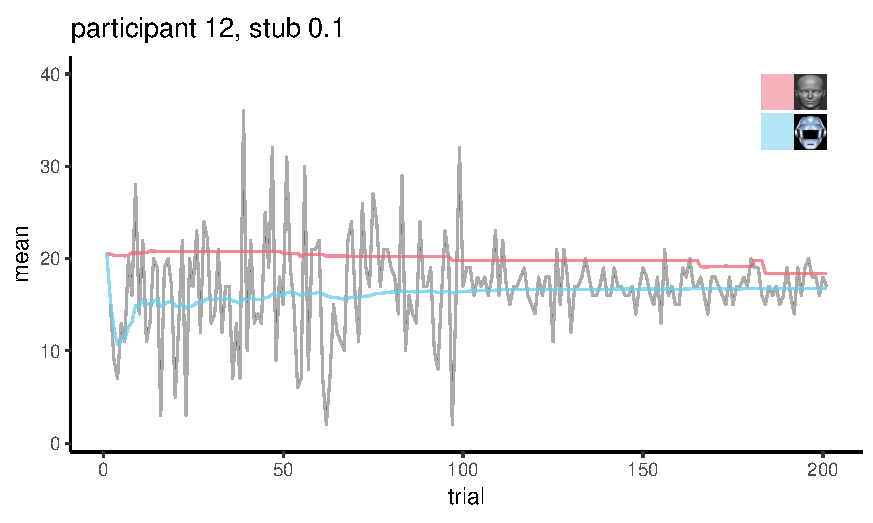
\includegraphics[width=\linewidth]{{comparisons1/means_12-stub_0.1}.pdf}
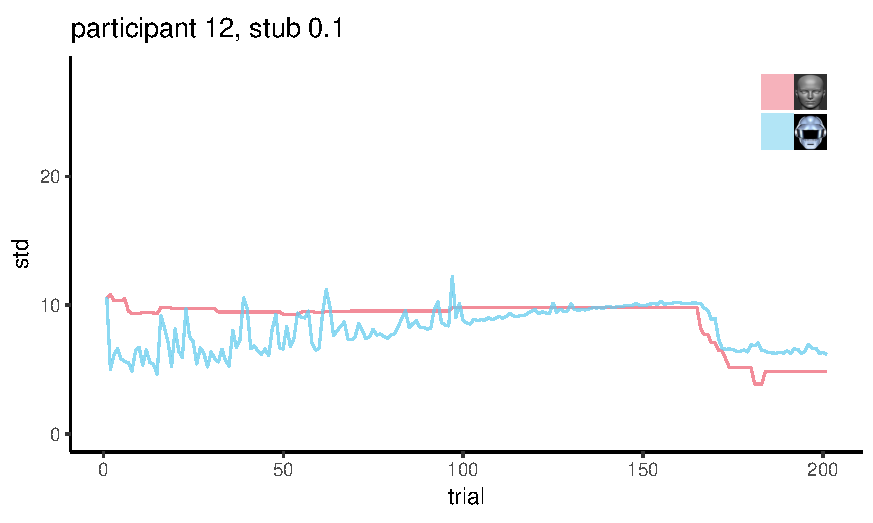
\includegraphics[width=\linewidth]{{comparisons1/stds_12-stub_0.1}.pdf}
\caption{Comparison of the means and standard deviations of the predictive
  distributions of participant~12 and of a robot with stubbornness
  $\yN=0.1$}\label{fig:comparison_12_01}
\end{figure}% done with exploration1.R
Figure~\ref{fig:comparison_12_01} shows the means and standard deviations
of the sequence such distributions, for participant~12 and a robot with
stubbornness $\yN=0.1$. This low value makes the robot give great
consideration to the first outcomes, as the initial high variability of the
robot's means shows. The algorithm generating the Plinko outcomes had a
change in standard deviation after the $100$th outcome, shifting to a
narrower distribution. The robot adapted to this change very slowly,
because it stubbornness at that point was $\yNo{100}\approx 100$.


\begin{figure}[p!]
\centering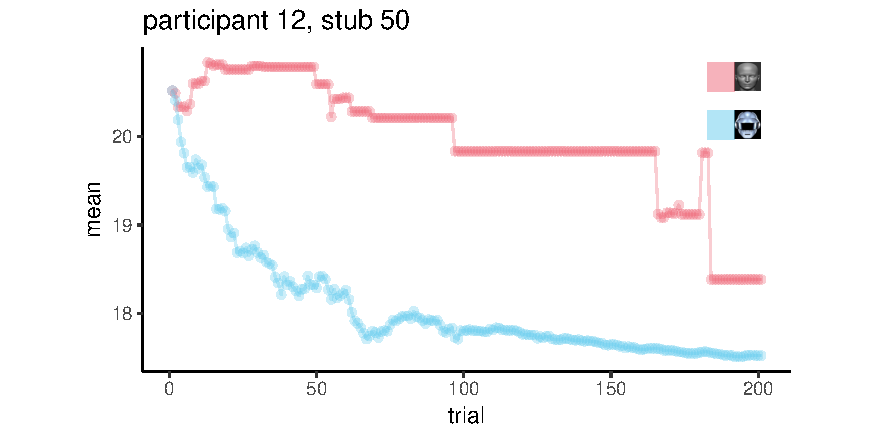
\includegraphics[width=\linewidth]{{comparisons1/means_12-stub_50}.pdf}
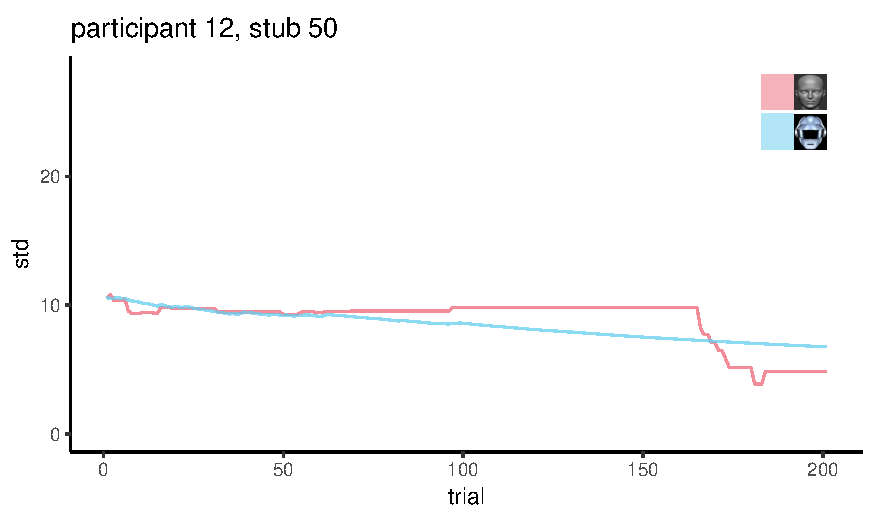
\includegraphics[width=\linewidth]{{comparisons1/stds_12-stub_50}.pdf}
\caption{Comparison of the means and standard deviations of the predictive
  distributions of participant~12 and of a robot with stubbornness
  $\yN=50$}\label{fig:comparison_12_50}
\end{figure}% done with exploration1.R
Figure~\ref{fig:comparison_12_50} is analogous to
\fig~\ref{fig:comparison_12_01} but for a robot with stubbornness
$\yN=50$. This robot is even more slow to adapt to the narrowing in the
standard deviation of the generated outcomes.


\begin{figure}[p!]
\centering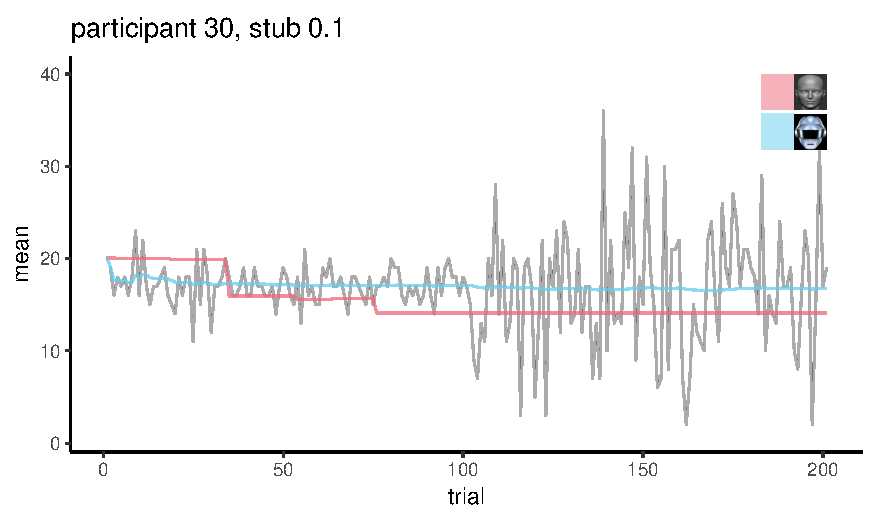
\includegraphics[width=\linewidth]{{comparisons1/means_30-stub_0.1}.pdf}
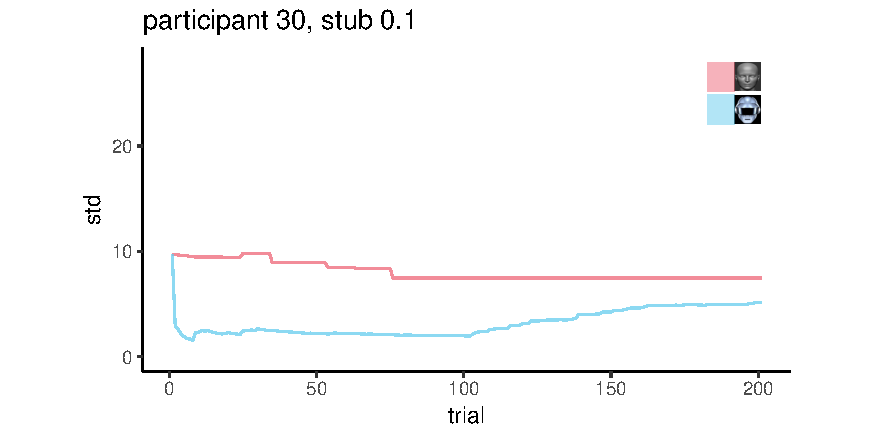
\includegraphics[width=\linewidth]{{comparisons1/stds_30-stub_0.1}.pdf}
\caption{Comparison of the means and standard deviations of the predictive
  distributions of participant~30 and of a robot with stubbornness
  $\yN=0.1$}\label{fig:comparison_30_01}
\end{figure}% done with exploration1.R
\begin{figure}[p!]
\centering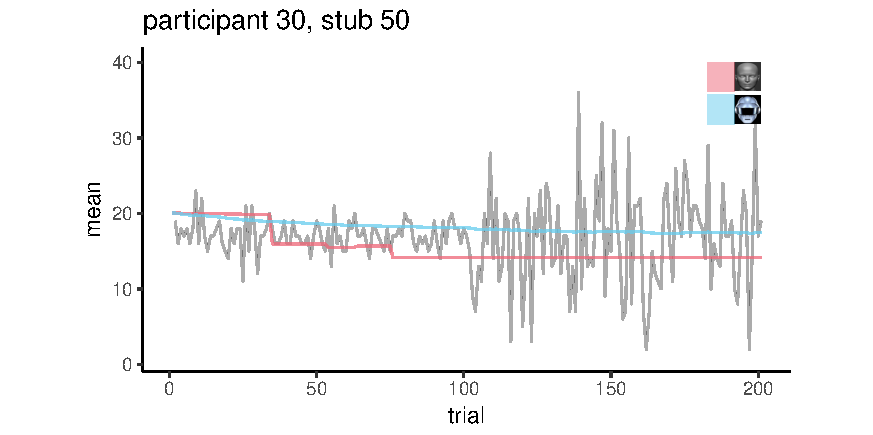
\includegraphics[width=\linewidth]{{comparisons1/means_30-stub_50}.pdf}
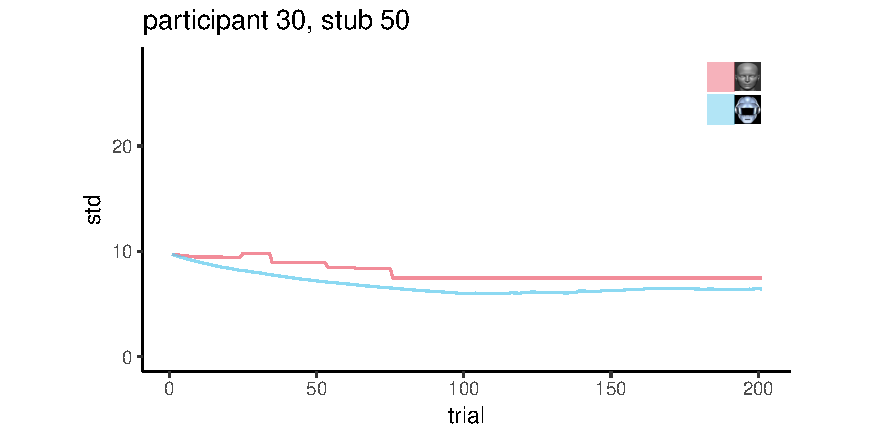
\includegraphics[width=\linewidth]{{comparisons1/stds_30-stub_50}.pdf}
\caption{Comparison of the means and standard deviations of the predictive
  distributions of participant~30 and of a robot with stubbornness
  $\yN=50$}\label{fig:comparison_30_50}
\end{figure}% done with exploration1.R
Figures~\ref{fig:comparison_30_01} and~\ref{fig:comparison_30_50} show
the same for participant~30. The change in standard deviation was from
narrow to large in this case.

The robot with low stubbornness seems to adapt to the widening of the
outcome outputs faster than it had for the narrowing of the previous case:
the change in the slope of the robot's standard-deviation curve seems
steeper in \fig~\ref{fig:comparison_30_01} than
in~\ref{fig:comparison_12_01}.


If we look at the sequence of outcomes of \figs~\ref{fig:comparison_12_01}
or~\ref{fig:comparison_30_01}, we perceive that something changed around
the $100$ observation. If we could plot these outcomes while they are
generated, we would likely notice the change by around the $25$th
observation. Our robot, however, can't detect this change for the reasons
explained in \sect~\ref{sec:remarks}; any outcomes from narrow or wide
generating processes are mixed in the robot's memory.

Only non-exchangeable or hierarchic statistical models, like the one we
develop in \sect~\ref{sec:second_study}, can exhibit a sort of memory for
the order and be capable of believing that the underlying
\enquote{mechanism} has changed.

\bigskip


Some conclusions can be drawn from the properties of our model and from the
examples:
\begin{itemize}[para]
\item Participants who have great inertia against updating their
  predictions in view of the observations are \emph{not} necessarily
  behaving at variance with the probability calculus. The latter says that
  they can be as stubborn as they please: larger $\yN$. If we judge such
  inertia as irrational, our judgement cannot be based on such a simple
  model; possibly it's based on a hierarchic model where $\yN$ is given a
  probability that depends on past experiences.

\item The slots have a specific physical order, and from the way the ball
  falls into them it seems reasonable to assume that updates to the
  probability for one slot should affect those for nearby slots. The
  Johnson-Dirichlet model does not take this into account. 

% \item A participant who, after observing outcome $k$, raises the bar under
%   that slot \emph{and nearby bars} is therefore not acting according to a
%   Johnson-Dirichlet exchangeable model.
\item Infinitely exchangeable priors are incapable of quickly adapting to
  changes in the empirical statistics of the outcomes.
\end{itemize}


\subsection{The robot's surprise}
\label{sec:examples_robot_surprise}

A robot with low stubbornness quickly adapts its predictions to the
observed outcomes, but as the outcomes accumulate its stubbornness
increases. If there is a late change in the generation of the outcomes,
after the $100$th observation for example, the robot will adapt its
predictions more slowly.

It is interesting to ask: is this prediction adaptation the same for a
change from a narrow to a wide distribution, as for a change from a wide to
a narrow one? or is there a difference in the adaptation speed?

The answer depends on how we measure such speed. One way could be this:
starting from the observation in which the change occurs, we let a second
robot with low stubbornness observe the new outcomes and make predictions,
starting from frequency parameters equal to those reached by the first
robot. The second robot will quickly adapt to the new observed outcomes,
and we can use it as a touchstone for the first robot's adaptation speed.
The predictions of the second robot can also be interpreted as if we had
reset the stubbornness of the first robot to a low value.

\begin{figure}[b!]
\centering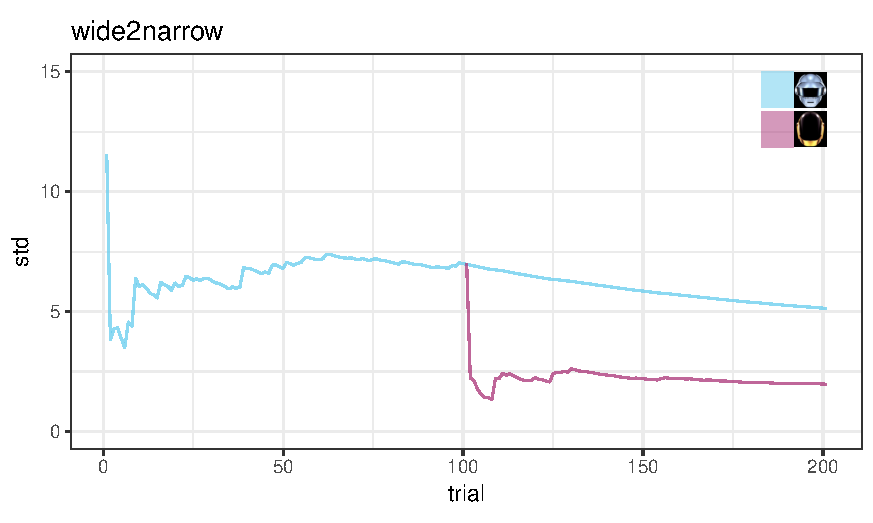
\includegraphics[width=\linewidth]{{comparisons1/compare_robots_wide2narrow-stub_0.1}.pdf}
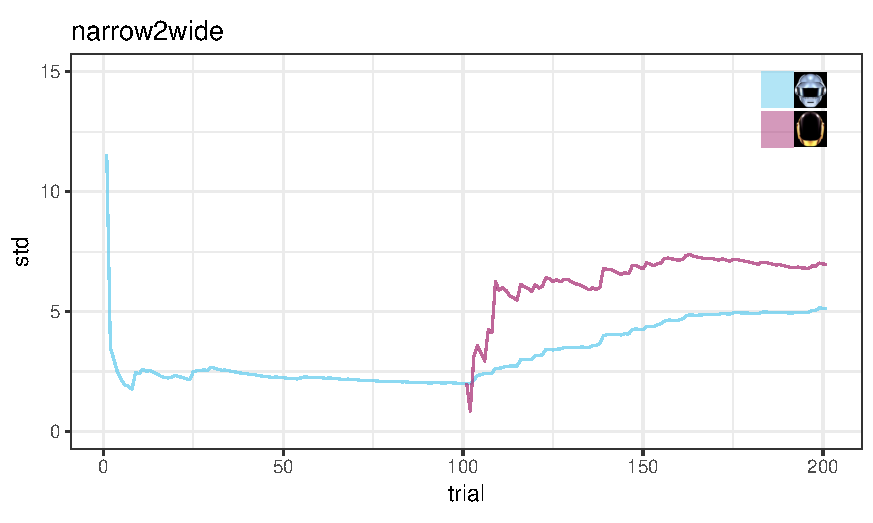
\includegraphics[width=\linewidth]{{comparisons1/compare_robots_narrow2wide-stub_0.1}.pdf}
\caption{Adaptation speed of the standard deviation for a robot after a
  change in the generation of the outcomes, compared with that of a robot
  that starts learning after the change. The final relative entropy for the
  first robot relative to the second is $1.01$ in the wide-to-narrow case,
  vs $0.260$ in the narrow-to-wide; exchanging the distributions: $0.283$
  vs $0.211$. The final normalized overlap is $0.949$ for wide-to-narrow vs
  $0.823$ for narrow-to-wide}\label{fig:comparison_robots_stds}
\end{figure}% done with exploration1.R
% wide2narrow: relentr=0.2825763, overlap=0.1059542
% narrow2wide: relentr=0.21082114, overlap=0.05119122
The results of this comparison are shown in
\fig~\ref{fig:comparison_robots_stds}. Looking at the standard deviations
of the distributions it seems that a robot adapts more slowly in going from
a wide to a narrow distribution than vice versa. This is true looking at
the final relative entropy of the first robot relative to the second:
$1.01$ wide-to-narrow vs $0.260$ narrow-to-wide; same if we exchange the
distributions: $0.283$ vs $0.211$. The overlap seems to say the
opposite: $0.106$ wide-to-narrow vs $0.0512$ narrow-to-wide; but the
overlap is heavily influenced by the narrowness of the overlapping
distributions, so it may not be a reliable measure in this case. If we use
the normalized overlap (corresponding to the cosine of the angle between
the distribution vectors) we find $0.949$ vs $0.823$, which agree with the
first three measures.

\begin{figure}[t!]
\centering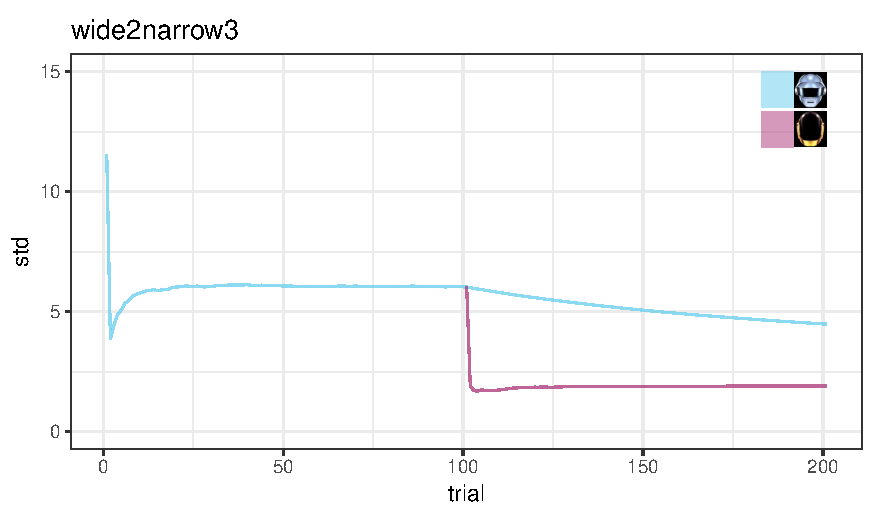
\includegraphics[width=\linewidth]{{comparisons1/avg_compare_robots_wide2narrow3-stub_0.1}.pdf}
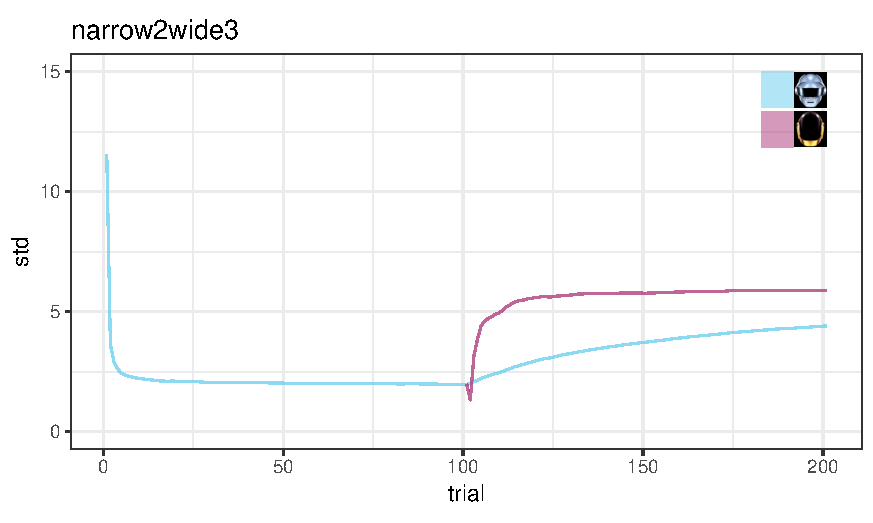
\includegraphics[width=\linewidth]{{comparisons1/avg_compare_robots_narrow2wide3-stub_0.1}.pdf}
\caption{Adaptation speed of the standard deviation for a robot after a
  change in the generation of the outcomes, compared with that of a robot
  that starts learning after the change, averaged over 100 experiments. The
  normals have same mean $17$ and standard deviations $6$ and
  $1.9$.}\label{fig:avg_comparison_robots_stds}
\end{figure}% done with exploration1.R
Figure~\ref{fig:avg_comparison_robots_stds} shows that this phenomenon is
even more striking if we average the sequences of standard deviations over
100 repetitions of such experiments.

\begin{figure}[b!]
\centering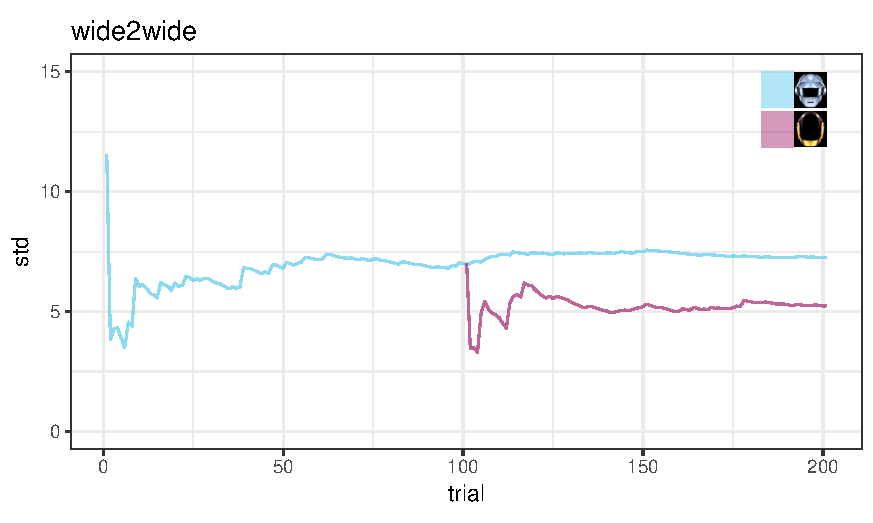
\includegraphics[width=\linewidth]{{comparisons1/compare_robots_wide2wide-stub_0.1}.pdf}
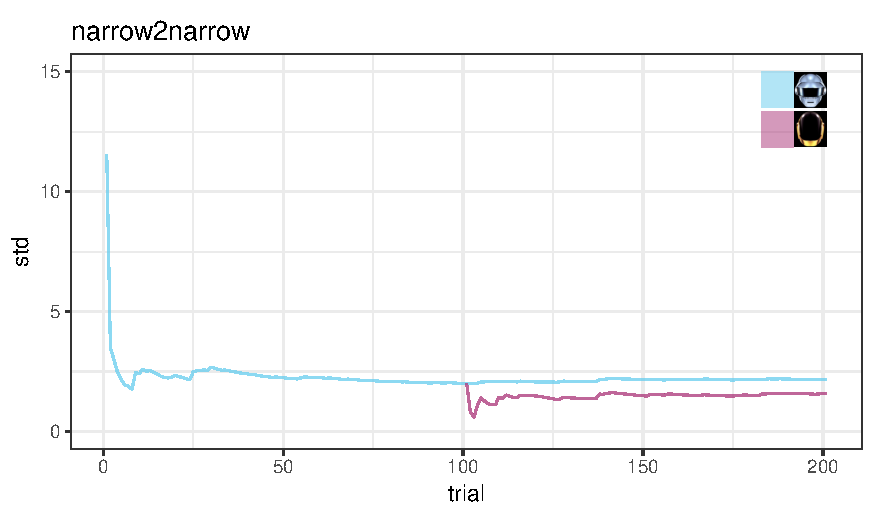
\includegraphics[width=\linewidth]{{comparisons1/compare_robots_narrow2narrow-stub_0.1}.pdf}
\caption{Adaptation speed of a robot after a change in the generation of
  the outcomes, compared with that of a robot that starts learning after
  the change.}\label{fig:comparison_robots_stds_2}
\end{figure}% done with exploration1.R

\clearpage

\section{Second study: Johnson-Dirichlet robots with change-points}
\label{sec:second_study}

\subsection{The robot looks for changepoints}
\label{sec:changepoints}

The robot of the previous study remembers past outcomes but not their
order. Said otherwise, it assumes that past frequencies are all that
matters for its inference. We now consider a new robot that takes the
outcome order into account in a simple way.

This new robot, denoted $\yMc$, is based on this assumption:
\begin{itemize}
\item the sequence of observations is divided into subsequences of
  contiguous observations. These subsequences can have different lengths.
  Within each subsequence, the order of the observations doesn't matter,
  and the Johnson-Dirichlet assumptions apply locally.
\end{itemize}
This robot therefore uses an infinitely exchangeable model with a
Johnson-Dirichlet parameter density for each subsequence, as in the
previous study. Only observations within a subsequence contribute to the
update of the distributions for the other observations in that subsequence.
Observations from other subsequences are ignored. As one subsequence ends,
the robot's initial-distribution parameter $\yn$ and stubbornness $\yN$ are
reset.

The robot doesn't know the changepoints in advance, however. Before each
observation, the robot first infers whether the observation belongs to a
new subsequence or it continues the previous one. In the first case, it
then infers the next outcome using a fresh Johnson-Dirichlet model. In the
second case, it infers the next outcome updating the parameters of Johnson
Dirichlet model used thus far. The final inference is a combination of
these two according to the law of total probability.

To translate these assumptions into probability distributions it's
convenient to introduce some propositions, denoted $R^{m}_{u}$, defined as
\begin{multline}
  \label{eq:def_prop_changepoint}
  \begin{aligned}
    R^{m}_{u}
    &\defd \text{\enquote{Only the previous $u$ outcomes are \textbf{r}elevant for the $m$th one}}
    \\
    &\equiv\text{\enquote{Observations $\set{m-u, m-u+1, \dotsc, m}$ form a subsequence}}
  \end{aligned}
  \\ \text{with $0\le u \le m-1$}.
\end{multline}
The equivalence of these two propositions should be clear from the
discussion above.

The proposition $R^{m}_{0}$, in particular, states that \emph{no} previous
observations are relevant for inferring the $m$th one; in other words, it
states that this observation is the start of a new subsequence.

For fixed $m$, the propositions $R^{m}_{u}$, $0\le u \le m-1$, are
obviously exhaustive (their probabilities sum to unity) and mutually
exclusive. The assumptions $\yMc$ made thus far imply that some
propositions for different $m$ are also exclusive:
\begin{gather}
  \label{eq:exclusive_across_m}
  \p(R^{m}_{u_{m}}, R^{m-1}_{u_{m-1}} \| \yMc) = 0
  \quad\text{if $u_{m}\ne 0$ and $u_{m} \ne u_{m-1}+1$},
\\\intertext{and therefore}
  \label{eq:exhaustive_R_from_previous}
  \p(R^{m}_{0} \| R^{m-1}_{v},\yMc) +
  \p(R^{m}_{v+1} \| R^{m-1}_{v},\yMc) = 1.
\end{gather}
The reason is that the $m$th outcome either starts a new subsequence, hence
$u_{m}=0$; or continues the current subsequence, which according to
$R^{m-1}_{u_{m-1}}$ contains the $(m-1)$th outcome and the previous
$u_{m-1}$ ones, and therefore $u_{m}=u_{m+1}+1$. All other cases are
impossible. Note that these other cases might be possible under assumptions
different from $\yMc$; they would represent a robot with a sort of
moving-window memory.

With these propositions about the changepoints, the reset rules described
above correspond to the following equalities, for all $m$:
\begin{multline}
  \label{eq:irrelevant_data_conditional_R}
  \p(\yO^{m}_{s_{m}} \|
  R^{m}_{u},  \yO^{m-1}_{s_{m-1}}, \dotsc, \yO^{1}_{s_{1}}, \yMc)
  ={}\\
  \begin{cases}
  \p(\yO^{m}_{s_{m}} \|
    R^{m}_{u},  \yO^{m-1}_{s_{m-1}}, \dotsc, \yO^{m-u}_{s_{m-u}}, \yMc)
    &\text{for $1\le u\le m-1$},
      \\
  \p(\yO^{m}_{s_{m}} \|
    R^{m}_{u}, \yMc)
    &\text{for $u=0$},
  \end{cases}
\end{multline}
Where the probabilities on the right side are given by the
Johnson-Dirichlet formulae~\eqref{eq:predictive_JD_general}
or~\eqref{update_params_JD}.

The formulae above lead to a conditional distribution for the $m$th outcome
given the previous ones only if the robot has been programmed with the
probabilities
\begin{equation}
  \label{eq:prob_R_conditional_only_data_before}
  \p(R^{m}_{u_{m}} \| \yO^{m-1}_{s_{m-1}},\dotsc, \yO^{1}_{s_{1}}, \yMc),
\end{equation}
which in turn can be obtained by marginalization and condizionalization
from the probabilities
\begin{equation}
  \label{eq:prob_R_conditional_before}
  \p(R^{m}_{u_{m}} \| \yO^{m-1}_{s_{m-1}}, R^{m-1}_{u_{m-1}},\dotsc,
  R^{2}_{u_{2}}, \yO^{1}_{s_{1}}, \yMc)
\end{equation}
for all legitimate $m$, $u_i$, and outcomes $s_i$. Additional assumptions
are necessary to determine the latter probabilities. For example, the
particular order of all past outcomes, the lengths of the previous
subsequences, or even the robot's previous distributions, and other factors
external to the experiment might all be relevant. The robot is programmed
with this assumption:
\begin{itemize}
\item only two quantities are relevant to infer whether the next
  observation starts a new subsequence: the total number $m-1$ of
  observations made so far, and the current length $v$ of the present
  subsequence.
\end{itemize}
In formulae this assumption is equivalent to a Markov property:
\begin{equation}
  \label{eq:prob_R_markov}
  \p(R^{m}_{u_{m}} \| \yO^{m-1}_{s_{m-1}}, R^{m-1}_{u_{m-1}},\dotsc,
  R^{2}_{u_{2}}, \yO^{1}_{s_{1}}, \yMc) =
  \p(R^{m}_{u_{m}} \|  R^{m-1}_{u_{m-1}}, \yMc).
\end{equation}
Recalling, \eqn~\eqref{eq:exhaustive_R_from_previous}, that only the values
$u_{m}=0$ and $u_{m}= u_{m-1}+1$ are possible, the conditional
probabilities above are summarized in the \emph{changepoint function}
\begin{equation}\label{eq:def_changepoint_function}
  \yrs(v,m)  \defd \p(R^{m}_{0} \|  R^{m-1}_{v}, \yMc),
  \qquad m \in\set{2,3,\dotsc}, \quad v\in\set{1,\dotsc,m-1}.
\end{equation}
It is the probability that the $m$th observation starts a new subsequence,
given that the previous subsequence had length $v$, including the $(m-1)$th
outcome (that's the reason for $v-1$ in the definition). Note that
from~\eqref{eq:exclusive_across_m}
\begin{equation}\label{eq:one_minus_h}
  \p(R^{m}_{v} \|  R^{m-1}_{v-1}, \yMc)  = 1-\yrs(v,m),\qquad v\ne 0.
\end{equation}
A little counting shows that the set of the possible changepoint functions,
for an experiment with $M$ observations, is $\clcl{0,1}^{(M^2-M)/2}$.

\medskip

Once we specify:
\begin{itemize}
\item the stubbornness $\yN$ and initial distribution $\yn$ to be used at
  each reset,
\item the changepoint function $\yrs(v,m)$,
\end{itemize}
our new robot $\yMc$ is completely programmed and can face the Plinko task.
Note that these specifications determine the joint
distribution~\eqref{eq:distr_statmodel}, through the assumptions made so
far.

\subsection{Online belief update}
\label{sec:online_update_2}

The beliefs of the Johnson-Dirichlet robot of \sect~\ref{sec:first_study}
during the Plinko task were fully summarized by $N$ independent parameters,
recursively updated online after each observation.

An analogous online update is possible for this robot, with some
differences: first, the number of parameters required increases linearly
with the observations; second, the updated parameter values depend on the
last outcome, on the parameter values before the last observation,
\emph{and} on some of the parameter values before the last but one
observation. The online-update algorithm we now develop follows closely
Adams \amp\ MacKay's \citey{adamsetal2007} but departs from it in some
important respects.


We first write probability for the $m$th observation given the previous
outcomes can be written
\begin{multline}
  \label{eq:prob_new_cond_R}
  \p(\yO^{m}_{s_{m}} \|
  \yO^{m-1}_{s_{m-1}}, \dotsc, \yO^{1}_{s_{1}}, \yMc)
  =
  \frac{\p(\yO^{m}_{s_{m}}, \yO^{m-1}_{s_{m-1}} \|
    \yO^{m-2}_{s_{m-2}},\dotsc, \yO^{1}_{s_{1}}, \yMc)}{
    \p(\yO^{m-1}_{s_{m-1}} \| \yO^{m-2}_{s_{m-2}}, \dotsc, \yO^{1}_{s_{1}}, \yMc)}
=  {}\\
  \frac{\sum\limits_{u=0}^{m-1}
  \p(\yO^{m}_{s_{m}} \|
  R^{m}_{u},  \yO^{m-1}_{s_{m-1}}, \dotsc, \yO^{m-u}_{s_{m-u}}, \yMc)
  \times
  \p(R^{m}_{u}, \yO^{m-1}_{s_{m-1}} \| \yO^{m-2}_{s_{m-2}} \dotsc, \yO^{1}_{s_{1}}, \yMc)}{
\p(\yO^{m-1}_{s_{m-1}} \| \yO^{m-2}_{s_{m-2}} \dotsc, \yO^{1}_{s_{1}}, \yMc)
}.
\end{multline}
The reason for taking $\yO^{m-1}_{s_{m-1}}$ out of the conditional argument
will be apparent in a moment. Note that the denominator is the probability
of the previous observation given the previous data: in a recursive
computation this would have been computed in the preceding step.

The products in the $u$ sum contain the term given
by~\eqref{eq:irrelevant_data_conditional_R}, which is just the
Johnson-Dirichlet conditional probability~\eqref{eq:predictive_JD_general},
and the joint probability for $(R^{m}_{u}, \yO^{m-1}_{s_{m-1}})$ given the
previous data. This joint probability can be decomposed introducing
$R^{m-1}_{v}$ for the previous observation:
\begin{multline}
  \label{eq:prob_R_and_last_decompose}
  \p(R^{m}_{u}, \yO^{m-1}_{s_{m-1}} \| \yO^{m-2}_{s_{m-2}}, \dotsc, \yO^{1}_{s_{1}}, \yMc) 
 ={} \\
  \frac{\sum_{v=1}^{m-1}
    \p(R^{m}_{u}, \yO^{m-1}_{s_{m-1}}, R^{m-1}_{v-1}, \yO^{m-2}_{s_{m-2}}
    \| \yO^{m-3}_{s_{m-3}}, \dotsc, \yO^{1}_{s_{1}}, \yMc)}{
\p(\yO^{m-2}_{s_{m-2}} \| \yO^{m-3}_{s_{m-3}}, \dotsc, \yO^{1}_{s_{1}}, \yMc)}
  ={}\\
    \frac{1}{\p(\yO^{m-2}_{s_{m-2}} \| \yO^{m-3}_{s_{m-3}}, \dotsc, \yO^{1}_{s_{1}}, \yMc)}
  \sum_{v=1}^{m-1} \p(R^{m}_{u} \| R^{m-1}_{v-1}, \yMc)
  \times{}\\
  \p(\yO^{m-1}_{s_{m-1}} \|
    R^{m-1}_{v-1}, \yO^{m-2}_{s_{m-2}} \dotsc, \yO^{m-v}_{s_{m-v}}, \yMc)
    \times{}\\
 \p(R^{m-1}_{v-1}, \yO^{m-2}_{s_{m-2}} \|
  \yO^{m-3}_{s_{m-3}},\dotsc, \yO^{1}_{s_{1}}, \yMc).
\end{multline}
The last expression contains four kinds of terms. Let's analyse them.

\begin{itemize}
\item The denominator is the probability for the $(m-2)$th observation
  given the previous data. In a recursive algorithm this is known from two
  previous steps.

\item The first factor within the $v$ sum was simplified using the Markov
  property~\eqref{eq:prob_R_markov}.

\item The second factor within the $v$ sum is given by the
  Johnson-Dirichlet model, according to discussion of
  \eqn~\eqref{eq:irrelevant_data_conditional_R}.

\item The last factor within the $v$ sum is analogous to the joint
  probability for $R^{m}_{u}, \yO^{m-1}_{s_{m-1}}$, which we are now
  calculating, but for the previous observation. In a recursive scheme it
  is known from the preceding step.
\end{itemize}

Combining formulae~\eqref{eq:prob_new_cond_R},
\eqref{eq:prob_R_and_last_decompose}, \eqref{eq:recursive_formula_2},
\eqref{eq:def_changepoint_function}, \eqref{eq:predictive_JD_general}, and
defining
\begin{subequations}\label{eq:definitions_ABC}
  \begin{align}
    \label{eq:def_A}
    A_{m}(s_{m}) &\defs
    \p(\yO^{m}_{s_{m}} \| \yO^{m-1}_{s_{m-1}}, \dotsc, \yO^{1}_{s_{1}}, \yMc),
    \\
    B_{m}(u,s_{m})
                 &\defd \p(\yO^{m}_{s_{m}} \| R^{m}_{u}, \yO^{m-1}_{s_{m-1}},
                   \dotsc, \yO^{m-u}_{s_{m-u}}, \yMc),
    \\
    C_{m}(u) &\defd
            \p(R^{m}_{u} , \yO^{m-1}_{s_{m-1}} \| \yO^{m-2}_{s_{m-2}}, \dotsc,
            \yO^{1}_{s_{1}}, \yMc),
  \end{align}
\end{subequations}
we find that the conditional probability we're seeking, $A_{m}(s_{m})$, is
given recursively by
\newlength{\myl}\settowidth{\myl}{\footnotesize the past $u$ observations}
\begin{subequations}\label{eq:recursive_formula_2}
\begin{align}
  A_{m}(s_{m})
  &= \frac{\sum_{u=0}^{m-1} B_{m}(u,s_{m}) \; C_{m}(u)}{A_{m-1}(s_{m-1})}
  \\
  B_{m}(u,s_{m})
  &= \frac{\yN\ynn_{s_{m}}+u\yff_{s_{m}}}{\yN + u},
    \qquad
    \yff_{s_{m}} \defd\Bigl\{
    \parbox[c]{\the\myl}{\footnotesize rel. frequency of $s_m$ in\\
  the past $u$ observations}
  \\
  C_{m}(u)
  &=   \!\begin{multlined}[t][0.6\linewidth]
    \frac{1}{A_{m-2}(s_{m-2})} \times{}\\[\jot]
    \begin{cases}
      \sum_{v=1}^{m-1} \yrs(v,m) \; B_{m-1}(v-1,s_{m-1}) \;
      C_{m-1}(v-1)
      & \text{if $u=0$}
      \\[\jot]
      [1-\yrs(u,m)]  \; B_{m-1}(u-1,s_{m-1}) \; C_{m-1}(u-1)
      & \text{if $u\ge 1$}
    \end{cases}
  \end{multlined}
\end{align}
\end{subequations}
for all $s_{m} \in\set{1,\dotsc,N}$, $u\in\set{0,\dotsc,m-1}$. This recursive
algorithm is summarized in table~\ref{tab:adamsetal_algorithm}.

\bigskip

Some initial values are necessary for this recursive scheme. For $m=1$, the
first observation, the distribution is $\p(\yO^{1}_{s_1} \| \yMc)=\ynn_{s_1}$
by the Johnson-Dirichlet model, and trivially $\p(R^{1}_{0} \| \yMc)=1$.
Owing to the certainty of $R^1_0$, for $m=2$ we have
\begin{equation}
  \label{eq:initial_R2}
  \p(R^{2}_{u}, \yO^{1}_{s_{1}} \|  \yMc)
  = \p(R^{2}_{u},R^{1}_{0}, \yO^{1}_{s_{1}} \|  \yMc)
  = \p(R^{2}_{u} \| R^{1}_{0},  \yMc) \times
  \p( \yO^{1}_{s_{1}} \|  \yMc).
\end{equation}
With the probabilities above from $m=3$ onward the recursion can be
calculated with \eqns~\eqref{eq:recursive_formula_2}. These initialization
steps are summarized in table~\ref{tab:adamsetal_initial}.

\begin{table}[!p]
  \centering
  \caption{Initial steps of predictive algorithm}
  \label{tab:adamsetal_initial}
  \begin{tabularx}{\textwidth}{X}\hline
    \begin{enumerate}%[label=0.\arabic*.,start=0]
    \item Assign numerical values to $\yN$, $\ynn$
    \item For $s_1 \in \set{1,\dotsc,N}$ calculate
      \[A_1(s_1)\defd \p(\yO^{1}_{s_{1}} \|  \yMc) =\ynn_{s_1} \]
    \item Observe $s_1$
    \item Keep  $A_1(s_1)$ for the next two steps and $B_1(0)\equiv 1$ for
      the next step

      \bigskip
    \item For $u \in\set{0,1}$:
      \begin{enumerate}[label*=\arabic*.]
   \item Calculate
      \[
        C_2(u) \defd \p(R^{2}_{u}, \yO^{1}_{s_1} \| \yMc)
        =
A_1(s_1) \times \begin{cases}
          \yrs(0,1) &\text{for $u=0$},\\ 1-\yrs(0,1)&\text{for $u=1$}
        \end{cases}
      \]
      \item For $s_{2} \in \set{1,\dotsc,N}$, calculate
        \[ 
          B_{2}(u,s_{2}) \defd
          \p(\yO^{2}_{s_{2}} \| R^{2}_{u}, \yO^{1}_{s_{1}}, \yMc) =
         \frac{\yN\ynn_{s_{2}}+u\yff_{s_{2}}}{\yN + u},
        \]
     where $\yff_{s_{2}}$ is the relative frequency of outcome $s_{3}$ in
     the previous $u$ observations
    \end{enumerate}
  \item  For $s_2 \in \set{1,\dotsc,N}$ calculate
      \[A_2(s_2) \defd
        \p(\yO^{2}_{s_{2}} \| \yO^{1}_{s_{1}}, \yMc) =
\frac{\sum_{u=0}^{1} B_{2}(u,s_{2}) \times C_{2}(u)}{A_{1}(s_{1})} \]
\item Observe $s_2$
\item Keep $A_{2}(s_{2})$ for the next two steps, and
  $B_{2}(u,s_{2})$, $C_{2}(u)$, $u\in\set{0,1}$, for the next step
\item Set $m=2$, go to step~\ref{item:first_step} of table~\ref{tab:adamsetal_algorithm}
\end{enumerate}
\\\hline
  \end{tabularx}
\end{table}

\begin{table}[!p]
  \centering
  \caption{Predictive algorithm}
  \label{tab:adamsetal_algorithm}
  \begin{tabularx}{\textwidth}{X}\hline
    \begin{enumerate}
      % \item Retrieve from memory
      %   \[ B_m(v) \defd \p(R^{m}_{v} \| \yO^{m-1}_{s_{m-1}} \dotsc,
      %     \yO^{1}_{s_{1}}, \yMc),\qquad 0\le v \le m-1 \]
    \item\label{item:first_step}For $u \in \set{0,\dotsc, m}$:
      \begin{enumerate}[label*=\arabic*.]
      \item Calculate
        \[ \begin{multlined}[t][0.85\textwidth]
            C_{m+1}(u) \defd
            \p(R^{m+1}_{u} , \yO^{m}_{s_{m}} \| \yO^{m-1}_{s_{m-1}}, \dotsc,
            \yO^{1}_{s_{1}}, \yMc) ={}\\[\jot]
       \shoveleft{\frac{1}{A_{m-1}(s_{m-1})} \times{}}\\\begin{cases}
          \sum_{v=0}^{m-1} \yrs(v,m) \times B_m(v,s_m) \times C_m(v) & \text{if $u=0$},
          \\[\jot]
          [1-\yrs(u-1,m)]  \times B_m(u-1,s_m) \times C_m(u-1)& \text{if $u\ge 1$}    
        \end{cases}
      \end{multlined}
    \]
      \item For $s_{m+1} \in \set{1,\dotsc,N}$, calculate
        \[ \begin{multlined}[][0.85\textwidth]
B_{m+1}(u,s_{m+1}) \defd \p(\yO^{m+1}_{s_{m+1}} \| R^{m+1}_{u}, \yO^{m}_{s_{m}},
          \dotsc, \yO^{m+1-u}_{s_{m+1-u}}, \yMc) ={}\\[\jot]
         \frac{\yN\ynn_{s_{m+1}}+u\yff_{s_{m+1}}}{\yN + u},
       \end{multlined} \]
     where $\yff_{s_{m+1}}$ is the relative frequency of outcome $s_{m+1}$ in the previous $u$ observations
      % \item using the Johnson-Dirichlet model calculate (or retrieve from memory)
      %   \[ A_m(v) \defd \p(\yO^{m}_{s_{m}} \| R^{m}_{v}, \yO^{m-1}_{s_{m-1}}
      %     \dotsc, \yO^{m-v}_{s_{m-v}}, \yMc)
      %   \]
  \end{enumerate}
\item For $s_{m+1} \in \set{1,\dotsc,N}$, calculate
  \[ \begin{multlined}[][0.85\textwidth]
      A_{m+1}(s_{m+1}) \defd \p(\yO^{m+1}_{s_{m+1}} \| \yO^{m}_{s_{m}}, \dotsc, \yO^{1}_{s_{1}}, \yMc) ={}\\[\jot]
    \frac{\sum_{u=0}^{m} B_{m+1}(u,s_{m+1}) \times
      C_{m+1}(u)}{A_{m}(s_{m})}
  \end{multlined}
\]
\item Observe $s_{m+1}$, 
\item Keep $A_{m+1}(s_{m+1})$ for the next two steps, and
  $B_{m+1}(u,s_{m+1})$, $C_{m+1}(u)$, $u\in\set{0,\dotsc,m}$ for the next step
\item Increase $m$ by $1$, go to step~\ref{item:first_step}
  \end{enumerate}
  \\\hline
\end{tabularx}
\end{table}

\subsection{Changepoint function and its uses}
\label{sec:changepoint_choice}

The changepoint function~\eqref{eq:def_changepoint_function},
\begin{equation}\labelbis{eq:def_changepoint_function}
  \yrs(v,m)  \defd \p(R^{m}_{0} \|  R^{m-1}_{v}, \yMc),
  \qquad m \in\set{2,3,\dotsc}, \quad v\in\set{1,\dotsc,m-1}
\end{equation}
determines the robot's inference about the appearance of changepoints, or
changes in the source of the data. It can represent a great
variety of changepoint assumptions or beliefs.

For example, the belief that the data source is the more likely to change
the longer it's been operative corresponds to a $\yrs$ that increases as
$v$ increases. The belief that the longer a data source operates the more
likely it will persist corresponds to a $\yrs$ that decreases as $v$
increases. Even more complex beliefs can be represented with the dependence
on $m$. For example, we can have a shift from the first to the second
belief above as $m$ increases.

Our new robot $\yMc$, thanks to this function, can reproduce a great
variety of human inferential behaviours. How well can such robots mimic
reproduce the inferential behaviour of the Plinko participants?

One way to assess this is to tune the stubbornness parameter $\yN$ and the
changepoint function $\yrs$ so that the robot's sequence of predictive
distributions is as close to a specific participant's as possible. The
reset-distribution parameter $\yn$ can be set equal to the participant's
initial distribution -- thus assuming that the participant would again
choose that distribution if he or she were informed about a change in the
algorithm determining the outcomes.

This optimization leads to a possibly unique set of parameters
$\bigl(\yN, \yrs(v,m)\bigr)$ associated to a participant. We could then
explore the distribution of these parameters across all participants, for
example examining whether they cluster into few groups, and so on.

For such a study we need to choose a measure of discrepancy between two
sequences of distributions, and to restrict our choice of changepoint
functions, to make the study computationally feasible. We now explore these
two necessities.

\subsection{Discrepancy between sequences of inferences}
\label{sec:discrepancy_measure}

There are many measures of the discrepancy between two distributions: the
relative entropy (also called Kullback-Leibler divergence or information
discrimination) of the first distribution with respect to the second; or of
the second with respect to the first; or the symmetrized version, namely the
Shannon-Jansen discrepancy; or the Hellinger distance; and many others.

Given such a discrepancy for each of the $M$ observations, we could define
the total discrepancy as the average of these ($L^1$ norm), or the maximum
among them ($L^{\infty}$ norm), or other similar measures.

\subsection{Restrictions on the changepoint function}
\label{sec:restrictions_h}

With $M$ observations, choosing a changepoint function corresponds to
choosing $(M^2-M)/2$ parameters with values in $\clcl{0,1}$. We try to
restrict this choice to make the optimization computationally feasible
while maintaining an enough wide range of changepoint beliefs.

One restriction is to specify a logistic-polynomial changepoint function
like this:
\begin{gather}
  \label{eq:changepoint_logistic_general}
  \yrs(v,m ; \gamma_0,\dotsc) =
  \logistic(\gamma_0 + \gamma_1 v + \gamma_2 m +
  \gamma_3 v^2 + \gamma_4  v m + \gamma_5 m^2 + \dotsb)
  \\
  \shortintertext{where the logistic function}
  \label{eq:logistic_def}
  \logistic(x) \defd \frac{1}{1+\e^{-x}} 
\end{gather}
maps real numbers to $\clcl{0,1}$.

In the rest of this study we choose a logistic-linear function:
\begin{equation}
  \label{eq:logistic_linear}
  \yrs(v,m; \yc,\ycs,\ycm) = \logistic\biggl( \yc +
  \ycs \frac{2 v-M}{M} + \ycm \frac{2 m-M}{M}\biggr) 
\end{equation}
thus reducing our choice to a three-parameter family of changepoint
functions. This family can reproduce, for example, the two simple kinds of
changepoint beliefs mentioned in \sect~\ref{sec:changepoint_choice}, but
not an $m$-dependent shift between them. Examples are shown in \fig***




\bigskip\mynote{Luca: work in progress in the rest of this subsection}


\clearpage

\section{Notes on hierarchic models}
\label{sec:notes_hierarchic}

\subsection{How hierarchic models get updated}
\label{sec:hierarchic_models}

The probability calculus allows for inferences that learn from data in
various degrees. We call \enquote{model} a particular way of doing
inference; each model is characterized by a particular capability of
learning from data. These capabilities arise from a hierarchy of groups
within groups of models.

At the bottom we have models that do not learn at all; we call them
\emph{independent}, because they assign independent probabilities to
different data. For example, denoting a particular independent model by
$\yth$ -- which could be the value of a parameter identifying the model --
and by $\yI$ all other knowledge or assumptions besides this model, we have
\begin{equation}
  \label{eq:indep_model}
  \pf(s_1,s_2 \| \yth, \yI) = \pf(s_1 \|\yth,\yI) \, \pf(s_2 \|\yth,\yI)
\end{equation}
for any two data $s_1$, $s_2$. This model does not learn because
\begin{equation}
  \label{eq:indep_model_nolearn}
  \pf(s_2\| s_1, \yth, \yI) = \pf(s_2 \|\yth,\yI),
\end{equation}
that is, under this model one set of data is always irrelevant for the
prediction of another set. The probability of an independent model given
data $s$ is
\begin{equation}
  \label{eq:prob_indep_model}
  \pf(\yth \| s, \yI)
  = \frac{
    \pf(s \|\yth,\yI) \, \pf(\yth \| \yI)
  }{
    \sum_{\yth}\pf(s \|\yth,\yI) \, \pf(\yth \| \yI)
  },
  % \equiv \frac{
  %   \pf(d \|\yth,\yI) \, \pf(\yth \| \yI)
  % }{
  %   \pf(d \|\yI)
  % },
\end{equation}
where $\pf(\yth \|\yI)$ is the probability over a range of such models
based only on knowledge $\yI$, and $\pf(s \|\yth,\yI)$ is the
\emph{likelihood} of the independent model given the data.

\medskip

We can introduce the capability of learning from data by considering a
collection $\set{\yth}$ of independent models, each having a probability,
and letting the data influence the probabilities of these models, rather
than the model themselves.

This particular model, based on a collection of independent models, is
usually called a \emph{parametric} model. Let us denote a particular
parametric model by $\ymu$. It is not independent because
\begin{equation}
  \label{eq:param_model}
  \begin{aligned}
  \pf(s_1,s_2 \| \ymu, \yI) &=
\sum_{\yth}
\pf(s_1,s_2 \|\yth,\ymu,\yI) \, \pf(\yth \| \ymu,\yI)
\\&\equiv
\sum_{\yth}
\pf(s_1 \|\yth,\ymu,\yI) \, \pf(s_2 \|\yth,\ymu,\yI)
 \, \pf(\yth \| \ymu,\yI),
  \end{aligned}
\end{equation}
which doesn't factorize unless $\pf(\yth \| \ymu,\yI)$ is a delta. The
first equality comes from the law of total probability. Such a model learns
because
\begin{subequations}
    \label{eq:param_model_learn}
  \begin{align}
    \pf(s_2 \| s_1, \ymu, \yI) &=
    \sum_{\yth}
    \pf(s_2 \|\yth,\ymu,\yI) \, \pf(\yth \| s_1, \ymu,\yI)
    \\
    \shortintertext{with}
    \pf(\yth \| s_1, \ymu,\yI)
    &= \frac{
      \pf(s_1 \|\yth,\ymu,\yI) \, \pf(\yth \| \ymu,\yI)
      }{
      \sum_{\yth} \pf(s_1 \|\yth,\ymu,\yI) \, \pf(\yth \| \ymu,\yI)
      },
  \end{align}
\end{subequations}
where we see that data $s_1$ affect not the probability of $s_2$ directly,
but the probability distribution for the various independent models. The
probability of a parametric model given data $s$ is
\begin{subequations}
  \label{eq:prob_indep_model}
  \begin{align}
    \pf(\ymu \| s, \yI)
    &= \frac{
      \pf(s \|\yth,\yI) \, \pf(\ymu \| \yI)
      }{
      \sum_{\ymu}\pf(s \|\ymu,\yI) \, \pf(\ymu \| \yI)
      }
    \\
    \shortintertext{with}
    \label{eq:param_model_likelihood}
    \pf(s \|\ymu,\yI)
    & =  
      \sum_{\yth}
      \pf(s \|\yth,\ymu,\yI) \, \pf(\yth \| \ymu,\yI).
  \end{align}
\end{subequations}
where $\pf(\ymu \|\yI)$ is the probability over a range of parametric
models based only on knowledge $\yI$. The last
expression~\eqref{eq:param_model_likelihood} is the \emph{likelihood} of
the model given the data, and we see that it's given by a mixture of
independent models.

\medskip

Equations~\eqref{eq:prob_indep_model} and~\eqref{eq:param_model} show that
a parametric model is constructed as an uncertainty over independent
models, and \eqn~\eqref{eq:param_model_learn} shows that data affect this
latter uncertainty. It is as if we were considering different ways of doing
inference, and inferring which of such inferences is most probable. Each
bottom inference is incapable to learn from data, but our inferences about
these inferences can learn from data.


We can proceed analogously and consider a collection $\set{\ymu}$ of
parametric models, each having a probability, and letting the data
influence this probability as well. The model constructed this way is
usually called a one-level hierarchic model -- even though we've seen that
a parametric model can also be considered as hierarchic. Let us denote such
a model by $\yh$. The probability of the data is
\begin{equation}
  \label{eq:hier_model}
  \begin{aligned}
  \pf(s_1,s_2 \| \yh, \yI) &=
\sum_{\ymu}
\pf(s_1,s_2 \|\ymu,\yh,\yI) \, \pf(\ymu \| \yh,\yI)
\\&\equiv
    \!\!\begin{multlined}[t][0.5\linewidth]
\sum_\ymu\biggl\{ \sum_{\yth}
\Bigl[ \prod_i\pf(s_i \|\yth,\ymu,\yh,\yI)\Bigr]\,
     \pf(\yth \| \ymu,\yh, \yI)\biggr\}\times{}\\
     \pf(\ymu \| \yh,\yI).
   \end{multlined}
  \end{aligned}
\end{equation}
Learning takes place this way:
\begin{subequations}
    \label{eq:hier_model_learn}
  \begin{align}
    \pf(s_2 \| s_1, \yh, \yI)
    &= \sum_{\ymu} \Bigl[\sum_{\yth}
      \pf(s_2 \|\yth,\ymu,\yh,\yI) \, \pf(\yth \| s_1, \ymu,\yh,\yI)
      \Bigr]\,
      \pf(\ymu \| s_1, \yh,\yI)
    \\
    \intertext{with}
      \begin{split}%[t][0.5\linewidth]
    \pf(\yth \| s_1, \ymu,\yh,\yI)
    &=\frac{
      \pf(s_1 \|\yth,\ymu,\yh,\yI) \, \pf(\yth \| \ymu,\yh,\yI)
      }{
      \sum_{\yth} \pf(s_1 \|\yth,\ymu,\yh,\yI) \, \pf(\yth \| \ymu,\yh,\yI)
    }
        \\[2\jot]
    &=\frac{
      \pf(s_1 \|\yth,\ymu,\yh,\yI) \, \pf(\yth \| \ymu,\yh,\yI)
      }{\pf(s_1 \| \ymu,\yh,\yI) },
    \end{split}\label{eq:update_h1}
      \\[3\jot]
    \pf(\ymu \| s_1, \yh,\yI)
    &= \frac{
      \pf(s_1 \|\ymu,\yh,\yI) \, \pf(\ymu \| \yh,\yI)
      }{
      \sum_{\ymu} \pf(s_1 \|\ymu,\yh,\yI) \, \pf(\ymu \| \yh,\yI)
      }.\label{eq:update_h2}
  \end{align}
\end{subequations}
Note that the denominator of the update formula~\eqref{eq:update_h1} for
$\yth$ is the updated probability~\eqref{eq:update_h2} for $\ymu$. Note
also that the space of independent models $\set{\yth}$ can be different for
different $\ymu$.

With a hierarchic model, it is as if we were considering different
\enquote{super-inferences} about ways of doing inferences, and inferring
which of such super-inferences is the most probable. This model learns from
the data in two ways: the data first give more probability to one or
another parametric model, and then give more probability to one or another
independent model within that parametric model. From another point of view
we can say that the data perform first a coarsen selection, and then a
finer one within each coarser selection.

We can of course multiply this kind of hierarchy ad libitum, proceeding as
we've done so far.

\subsection{Flattening hierarchic models}
\label{sec:flatten}

The subdivision of learning into two or more levels of different coarseness
can be very convenient, but mathematically it's always equivalent to one single
subdivision at the finest level. In other words, any hierarchic model can
always be rewritten as a parametric one. Let's see how, in the case of a
hierarchic model like~\eqref{eq:hier_model}.

We said that each parametric model $\ymu$ has a set
$\set{\yth} = \set{\yth}_{\ymu}$ of underlying independent models. For
example, in the case of real-valued data, one set could contain normal
distributions with the same variance and different means; another set could
contain uniform distributions with different supports; yet another set
could contain Cauchy distributions with the same location parameter and
different scale parameters. These sets can be pairwise disjoint,
overlapping, or even identical for different $\ymu$.

First of all let's consider each such set $\set{\yth}_{\ymu}$ as formally
distinct from all others for different $\ymu$. We consider the union of all
these sets, denoting a member of this union by $\yTh$:
\begin{equation}
  \label{eq:union_indip_models}
  \set{\yTh} \defd \bigcup_{\ymu}\set{\yth}_{\ymu}.
\end{equation}
Now consider the predictive probability~\eqref{eq:hier_model} for the
hierarchic model:
\begin{equation}
  \label{eq:hier_model_simple}
  \pf(s \| \yh, \yI) =
\sum_\ymu\biggl[ \sum_{\yth}
\pf(s \|\yth,\ymu,\yh,\yI)\,
     \pf(\yth \| \ymu,\yh, \yI)\biggr]\,
     \pf(\ymu \| \yh,\yI).
\end{equation}
If we decree that $\pf(\yTh \| \ymu,\yh,\yI) = 0$ if $\yTh \notin
\set{\yth}_{\ymu}$, we can extend the sum over $\yth$ (for fixed $\ymu$)
over all $\yTh$. Moreover, since $\yTh$ contains information about $\ymu$,
the latter becomes irrelevant in the conditional of the probability $\pf(s
\|\yth,\ymu,\yh,\yI)$. The predictive probability above then becomes
\begin{equation}
  \label{eq:hier_model_Theta}
  \begin{split}
  \pf(s \| \yh, \yI) &=
\sum_{\yTh}
\pf(s \|\yTh,\yh,\yI)\, \sum_\ymu 
     \pf(\yTh \| \ymu,\yh, \yI)\,
     \pf(\ymu \| \yh,\yI),
\\ &= \sum_{\yTh}
\pf(s \|\yTh,\yh,\yI)\,
     \pf(\yTh \| \yh, \yI),
   \end{split}
\end{equation}
where the last equality follows from the law of total probability. What's
important in the last formula is that the probability
$\pf(s \|\yTh,\yh,\yI)$ factorizes over conjunctions of data; that is, it
is an independent model. The model above is therefore just a parametric
model.

The last step consists in joining together into a single value all those
values of $\yTh$ which lead to identical predictive distributions
$\pf(s \|\yTh,\yh,\yI)$. The probability $\pf(\yTh \| \yh, \yI)$  for such
a value will be the sum of the probability for the various equivalent values.

\mynote{to be cont'd}



%\setlength{\intextsep}{0.5ex}% with wrapfigure
%\begin{figure}[p!]%{r}{0.4\linewidth} % with wrapfigure
%  \centering\includegraphics[trim={12ex 0 18ex 0},clip,width=\linewidth]{maxent_saddle.png}\\
%\caption{***}\label{fig:comparison_a5}
%\end{figure}% exp_family_maxent.nb


\iffalse
\begin{acknowledgements}
  \ldots to Mari \amp\ Miri for continuous encouragement and affection, and
  to Buster Keaton and Saitama for filling life with awe and inspiration.
  To the developers and maintainers of \LaTeX, Emacs, AUC\TeX, Open Science
  Framework, Python, Inkscape, Sci-Hub for making a free and unfiltered
  scientific exchange possible.
%\rotatebox{15}{P}\rotatebox{5}{I}\rotatebox{-10}{P}\rotatebox{10}{\reflectbox{P}}\rotatebox{-5}{O}.
%\sourceatright{\autanet}
\end{acknowledgements}
\fi

%\appendixpage
%\appendix

%%%%%%%%%%%%%%% BIB %%%%%%%%%%%%%%%

\defbibnote{prenote}{{\footnotesize (\enquote{de $X$} is listed under D,
    \enquote{van $X$} under V, and so on, regardless of national
    conventions.)\par}}
% \defbibnote{postnote}{\par\medskip\noindent{\footnotesize% Note:
%     \arxivp \mparcp \philscip \biorxivp}}

\printbibliography[prenote=prenote%,postnote=postnote
]

\end{document}
---------- cut text ----------------




The observations at which the subsequences start, called changepoints, are
guessed from the whole sequence of observations. The robot is effectively
considering all possible numbers and positions of changepoints. For
example, every observation could be a subsequence by itself, or all
observations could belong to just one subsequence -- which was the
assumption of the robot of the previous study. According to Bayes's
theorem, the robot assigns a probability to each possible division
proportionally to a prior times the product of the probabilities for the
data in each subsequence determined by that division, calculated with the
Johnson-Dirichlet model described above:
\begin{multline}
  \label{eq:explanation_P_group}
  \p(\ptext{particular division into subsequences} \| \ptext{data}, \yMc)
  \propto{}\\
\colorlet{savedcolor}{.}
\color{gray}
\protect\parbox[c][][u]{0.2\linewidth}{\footnotesize each is a\\[0.5\jot]Johnson-Dirichlet\\[0.5\jot]model}\color{gray}\left\{\color{savedcolor}\;
    \!\begin{aligned}
        &\p(\ptext{data in 1st subsequence} \|
          \ptext{particular division}, \yMc)\times{}
          \\
        &\p(\ptext{data in 2nd subsequence} \|
          \ptext{particular division}, \yMc)\times{}
          \\
              &\dotsm\times{}
  \end{aligned}\right.\\
 \p(\ptext{particular division} \| \yMc),
\end{multline}
where $\yMc$ stands for other background assumptions. The final inference is
a combination of the inferences conditional on each possible division:
\begin{multline}
  \label{eq:explanation_group_mixed}
  \p(\ptext{new observation} \| \ptext{data}, \yMc) \propto{}\\[\jot]
  \sum_{\mathclap{\text{all divisions}}}
  \p(\ptext{new observation} \| \ptext{division}, \ptext{data}, \yMc)
\times  \p(\ptext{division} \| \ptext{data}, \yMc),
\end{multline}
where the probability for the new observation given the division is
determined by the Johnson-Dirichlet model.

According to this assumption, past observations help us guessing whether
the next observation starts a new subsequence only if we can compare them
with it. If we don't know it, past data can't help us. This assumption
discards the possibility that particular values of past observations may
trigger the start of a new sequence. The length of the current subsequence,
$R^{m}_{v}$, is relevant in any case, because the next observation can only
start a new subsequence or continue the previous one, so that either $u=0$
or $u=v+1$:
\begin{equation}
  \label{eq:R_cond_R_simple}
  \p(R^{m+1}_{u} \| R^{m}_{v}, \yMc) =
  \yrs(v,m)\,\delt_{u,0} + [1-\yrs(v,m)]\,\delt_{u,v+1} =
  \begin{cases}
    \yrs(v,m) & \text{for $u=0$},
    \\
    1-\yrs(v,m) &\text{for $u=v+1$},
    \\
    0 & \text{otherwise},
  \end{cases}
\end{equation}
which simplifies our calculations: in the
sum~\eqref{eq:prob_R_and_last_decompose} when $u\ge 1$ only the term
$v=u-1$ survives. In our study we assume that $\yrs(v,m)$ either is
independent of $v$ or increases with $v$, expressing our expectation that
subsequences shouldn't be too long. This last option is reasonable if the
participants were warned about the possibility of changepoints before the
experiment.

% This distribution for $R^{m+1}_u$ represents the robot's guess of whether
% the new observation starts a new subsequence or whether it is part of the
% previous subsequence, and of how long that subsequence is. It can be
% calculated recursively by introducing $R^{m}_{v}$ for the previous
% observation:
% \begin{equation}
%   \label{eq:prob_R_and_last_decompose2}
%     \p(R^{m+1}_{u}\| \yO^{m}_{s_{m}}, \dotsc, \yO^{1}_{s_{1}}, \yI) 
%   % &=\sum_{v=0}^{m-1}
%   % \p(R^{m+1}_{u},R^{m}_{v},\|
%   % \yO^{m}_{s_{m}}, \dotsc, \yO^{1}_{s_{1}}, \yI)
%   % \\
% =\sum_{v=0}^{m-1}\p(R^{m+1}_{u} \| R^{m}_{v}, \yI)
%   \times
%   \p(R^{m}_{v} \|
%   \yO^{m-1}_{s_{m-1}} \dotsc, \yO^{1}_{s_{1}}, \yI).
% % &\!\begin{multlined}[b][0.7\textwidth]
% %   =\sum_{v=0}^{m-1}\p(R^{m+1}_{u} \| R^{m}_{v}, \yI)
% %   \times{}\\
% %   \p(\yO^{m}_{s_{m}} \| R^{m}_{v},
% %   \yO^{m-1}_{s_{m-1}} \dotsc, \yO^{m-v}_{s_{m-v}}, \yI)
% %   \times{}\\
% %   \p(R^{m}_{v} \|
% %   \yO^{m-1}_{s_{m-1}} \dotsc, \yO^{1}_{s_{1}}, \yI).
% %           \end{multlined}
% %   \end{aligned}
% \end{equation}
% Let's examine the two factors in the sum.

%%% Local Variables: 
%%% mode: LaTeX
%%% TeX-PDF-mode: t
%%% TeX-master: t
%%% End: 
